% Isaac Dunn Part II Computer Science Dissertation
\documentclass[12pt,a4paper,twoside,openright]{report}
\usepackage[pdfborder={0 0 0}]{hyperref}    % turns references into hyperlinks
\usepackage[margin=25mm]{geometry}  % adjusts page layout
\usepackage[T1]{fontenc}
\usepackage{mathpazo}  % style
\usepackage{graphicx}  % allows inclusion of PDF, PNG and JPG images
\graphicspath{ {./figs/} }
\DeclareGraphicsExtensions{.pdf,.png,.jpg}
\usepackage{verbatim}
\usepackage{docmute}   % only needed to allow inclusion of proposal.tex
\usepackage{amsmath}
\usepackage{amsfonts}
\usepackage{algorithm}
\usepackage[noend]{algpseudocode}
\usepackage{enumitem}
\usepackage{color}
\usepackage{listings}
\usepackage{subcaption}
\usepackage[labelfont=bf]{caption}

\definecolor{dkgreen}{rgb}{0,0.6,0}
\definecolor{grey}{rgb}{0.5,0.5,0.5}
\definecolor{mauve}{rgb}{0.58,0,0.82}
\lstset{ % style of code listings
	frame=tb,
	language=ML,
	aboveskip=3mm,
	belowskip=3mm,
	showstringspaces=false,
	columns=flexible,
	basicstyle={\small\ttfamily},
	numbers=none,
	numberstyle=\tiny\color{grey},
	keywordstyle=\color{blue},
	commentstyle=\color{dkgreen},
	stringstyle=\color{mauve},
	breaklines=true,
	breakatwhitespace=true,
	tabsize=4
	}


\raggedbottom                           % try to avoid widows and orphans
\sloppy
\clubpenalty1000%
\widowpenalty1000%

\renewcommand{\baselinestretch}{1.1}    % adjust line spacing to make
                                        % more readable

% "let a = b in" for use in algorithms
\newcommand{\Let}[2]{\State \textbf{let} #1 = #2 \textbf{in}}

% For use in the happens-before relation varient
\newcommand{\longhookrightarrow}
	{\ensuremath{\lhook\joinrel\longrightarrow}}


\newenvironment{understandinglist}
	{\begin{itemize} \itemsep 0em}{\end{itemize}}
\begin{document}

\bibliographystyle{plain}


%%%%%%%%%%%%%%%%%%%%%%%%%%%%%%%%%%%%%%%%%%%%%%%%%%%%%%%%%%%%%%%%%%%%%%%%
% Title page


\pagestyle{empty}

\rightline{\LARGE \textbf{Isaac Dunn}}

\vspace*{60mm}
\begin{center}
\Huge
\textbf{Dynamic Partial-Order Reduction for Model Checking} \\[7mm]
Computer Science Tripos -- Part II \\[6mm]
Clare College \\[7mm]
\LARGE \today  % today's date
\end{center}

%%%%%%%%%%%%%%%%%%%%%%%%%%%%%%%%%%%%%%%%%%%%%%%%%%%%%%%%%%%%%%%%%%%%%%%%%%%%%%
% Proforma, table of contents and list of figures

\pagestyle{plain}

\chapter*{Proforma}

{\large
\begin{tabular}{ll}
Name:           & \bf Isaac Dunn                            			 \\
College:        & \bf Clare College                    				     \\
Project Title:	& \bf Dynamic Partial-Order Reduction for Model Checking \\
Examination:    & \bf Computer Science Tripos -- Part II, June 2016      \\
Word Count:     & \bf N    												 \\
Project Originator: & \bf Isaac Dunn\footnotemark[1] 					 \\
Supervisors:	& \bf Dr. Jonathan Hayman \& Prof. Glynn Winskel         \\
\end{tabular}
}
\footnotetext[1]{with guidance from Dr. Jonathan Hayman}
\stepcounter{footnote}


\section*{Original Aim of the Project}

The original aim of the project was to build a system which
used dynamic partial-order reduction to improve the performance
of a model checking algorithm which could be used to find
assertion violations and deadlocks.

\section*{Work Completed}

The original aim of the project was met and exceeded, with
a stateful implementation of dynamic partial-order reduction
also being produced.

\section*{Special Difficulties}

No special difficulties were encountered, only the usual dozens of
difficult-to-find bugs.
 
\newpage
\section*{Declaration}

I, Isaac Dunn of Clare College, being a candidate for Part II of the Computer
Science Tripos, hereby declare
that this dissertation and the work described in it are my own work,
unaided except as may be specified below, and that the dissertation
does not contain material that has already been used to any substantial
extent for a comparable purpose.

\bigskip
\leftline{Signed:}

\bigskip
\leftline{Date:}

\tableofcontents

\listoffigures

\newpage
\section*{Acknowledgements}

Put acknowledgements here.

%%%%%%%%%%%%%%%%%%%%%%%%%%%%%%%%%%%%%%%%%%%%%%%%%%%%%%%%%%%%%%%%%%%%%%%
% now for the body

\pagestyle{headings}

\chapter{Introduction}
After reading this chapter,
you should understand:
\begin{understandinglist}
	\item what model checking is and why it is useful;
	\item what the state explosion problem is;
	\item how partial-order reduction
	techniques address the state explosion problem;
	\item the aims of my project; and
	\item the aims of this dissertation.
\end{understandinglist}

\section{Model Checking}
After reading this section,
you should understand why formal methods for
verifying the correctness of software and
hardware systems are useful, that model
checking is such a formal method, and
how model checking works.

We want to be very sure that some computer
programs are correct. Testing is not good
enough -- all software products have been
tested, but according to Dijkstra,
\emph{``Testing shows the presence,
	not the absence, of bugs''}.

Model checking is a category of formal
methods, in which \textbf{(basic explanation of
model checking)}

\section{The State Explosion Problem}
After reading this section, you should
understand what the state explosion problem
is, and its practical implications.

Concurrent software programs in practice often
use threads as their model. The number of possible
interleavings of concurrent threads blows up very 
quickly.

Give some maths, some empirical results,
and a state space diagram showing this.

\section{Partial-Order Reduction}
After reading this section, you should
understand how partial-order reduction
techniques aim to address the state
explosion problem.

Idea: some interleavings are equivalent. If you
can identifying which are equivalent, you only
have to explore a subset. \emph{Give picture.}

Partial-order reduction is a category of techniques
that aim to identify such equivalences and so
perform model checking more efficiently.

\section{Dynamic Partial-Order Reduction}
After reading this section, you should
understand the idea behind the dynamic
partial-order reduction algorithm.

DPOR uses runtime information to identify
equivalent interleavings. In fact, it assumes
that all interleavings are equivalent, picks
one arbitrarily, and takes note of backtracking
points which might lead to un-equivalent
interleavings, which are then explored on
backtrack.

\section{This Project}
After reading this section, you should
understand the aims of my project,
my motivation for deciding on this
project, and have a shallow
understanding of its success.

The aim of this project is to implement DPOR.

It succeeded, and went further, implementing
a stateful version of DPOR, in which a table
of visited states is kept, and when a state is
re-visited, it is not re-explored. However, care
must be taken to make sure that this approach is
sound.

I chose this project to see how theory is
implemented in practice.

\section{Summary}
Having read this chapter,
you should now understand:
\begin{understandinglist}
	\item that model checking is a formal
	technique used to verify the correctness
	of programs;
	\item that model checking can be used in
	practice to find bugs in software and hardware
	implementations, and to provide evidence of
	correctness;
	\item that the state explosion problem is the
	exponentially increasing time required to model
	check concurrent programs, as the number and
	complexity of threads increases;
	\item that partial-order reduction and other
	techniques aim to address the state explosion
	problem by exploring only a sufficient subset
	of the state space of a given program;
	\item that my project aimed to implement a
	simple concurrent programming language
	and the dynamic partial-order reduction
	algorithm to perform model checking for
	programs in that language; and
	\item that this dissertation aims to give
	you an understanding of the work I have done,
	and of the relative merits of algorithms
	aiming to address the state space problem.
\end{understandinglist}

\chapter{Preparation}
After reading this chapter,
you should understand:
\begin{understandinglist}
	\item the precise definitions of the
	mathematical objects on which model
	checking is performed, in the context
	of my project;
	\item exactly what I mean by model checking
	in the context of this project, and therefore
	exactly what the aim of my project was;
	\item how a simple model checking algorithm
	works;
	\item exactly how the techniques of persistent sets
	and sleep sets address the state explosion
	problem;
	\item exactly how the dynamic partial-order
	reduction algorithm operates; and
	\item \emph{the work I undertook before beginning
	the implementation of my project.}
\end{understandinglist}

\subsubsection{Old Introduction}
The main preparation that was necessary before
the implementation of the project was the
development of a firm understanding of an
area of computer science that was new to me,
and in particular an understanding of the
DPOR algorithm itself. This was achieved
by study of the literature -- I began with
the paper introducing DPOR, and mostly
recursively followed references.

This chapter gives an overview of
the theoretical background, states precisely
what I mean by model checking, and briefly
introduces the DPOR algorithm.

\section{Background Definitions} \label{sec:background-defs}
After reading this section, you should understand the
formal definitions of the mathematical objects
which are manipulated by the algorithms used in
this project, \emph{as well as having an intuition for
what each mathematical object refers to in practice}.

\subsection{Processes and States}
We consider a system consisting of a finite set, $\mathcal{P}$,
of concurrent threads or processes (I use ``thread" and
``process" interchangeably throughout).
Each thread has its own local state, $s \in \mathcal{S}$, and there
is some shared global state, $g \in \mathcal{G}$. The overall
state of the system at any instant is therefore a member of the set
$ \textit{State} = (\mathcal{P} \to \mathcal{S}) \times \mathcal{G} $.

Each process executes a sequence of operations, as
specified in some programming language, each of which can
operate on the thread's local state $s$ or the shared
state $g$. If an operation
operates on $g$, it is said to be \emph{visible}, else it is said to be
\emph{invisible}.

\subsection{Transitions}
A \emph{transition} moves the system from one state to another,
by performing a finite sequence of invisible operations of some
process $p$, followed by a visible operation of the same process.
If process $p$ has local state $s$, then the transition $t_{p,s}$
that $p$ can make is defined to be a partial function taking the current
global state $g$ and giving $(s', g')$, the next local state for $p$
and the next global state for the system. Let $\mathcal{T}$ denote the
set of all transitions, so that
	\[\mathcal{T} = \mathcal{G} \rightharpoonup
				(\mathcal{S} \times \mathcal{G}).\]

A transition $t_{p,s}$ is said to be \emph{enabled} in a state
$(l, g)$ if and only if $l(p) = s$ and $t_{p,s}(g)$ is defined.
If $t_{p,s}$ is enabled in $\sigma = (l, g)$ and 
$t_{p,s}(g) = (s', g')$, then we say that the
execution of $t_{p,s}$ from $\sigma$ results in the unique successor
state $\sigma' = (l', g')$, where

\[
	l'(q) = \left\{\begin{array}{lr}
				s' & \textmd{if } p = q, \\
				l(q) &\textmd{if } p \neq q.
			\end{array} \right.
\]
In this case we write $\sigma \xrightarrow{t_{p,s}} \sigma'$.
We write $\longrightarrow^*$ to denote the transitive reflexive
closure of $\longrightarrow$.
A state $\sigma$ is called a \emph{stopped state} when there is no transition
$t$ such that $t$ is enabled in $\sigma$. We say that $t_1$ and $t_2$
may be \emph{co-enabled} if there is some state $\sigma \in \textit{State}$
such that both $t_1$ and $t_2$ are enabled in $\sigma$.

In any state $\sigma = (l, g)$, let
$\textit{next}(\sigma, p) = t_{p,l(p)}$ denote the unique next transition
to be executed by process $p$, and let
\[
	\textit{enabled}(\sigma) = \{t_{p,s} \in \mathcal{T} \mid
	p \in \mathcal{P} \wedge t_{p,s} = \textit{next}(\sigma, p)
	\wedge t_{p,s} \text{ is enabled in } \sigma\}
\]
denote the set of enabled transitions that can be executed from $\sigma$.
For any transition $t_{p,s}$, let $\textit{proc}(t_{p,s}) = p$
denote the unique process executing that transition.

\subsection{Systems}
The behaviour of an entire \emph{transition system} is
specified with the tuple $A = (\textit{State}, \Delta, \sigma_0)$,
where $\Delta \in State \to \mathbb{P}(State)$
is the \emph{transition relation} defined by
\[
	\sigma' \in \Delta(\sigma) \iff
	\exists t \in \mathcal{T}. \ \sigma \xrightarrow{t} \sigma'.
\]
Note that transitions are also known as models,
so model checking is the process of deciding
whether a given transition system has certain
properties.

\section{Model Checking}
After reading this section, you should
understand exactly what I mean by a
model-checking algorithm in the context
of this project, \emph{how this relates to
requirements analysis and the aims
of the project}, and how a simple
model-checking algorithm works.

\subsection{Definition of Model Checking}
\label{sec:model-checking-dfn}
Model checking is the process of deciding
whether a
given transition system is \emph{error-free} and
\emph{deadlock-free}.

To specify exactly what it means for a system to
be error-free, we extend each transition system
with a relation
$\textit{err} : \mathcal{S} \to \mathbb{B}$, which states
whether, in some given state, a particular
thread has encountered an error.

We say that a transition system
$A = (\textit{State},\, \Delta,\, \sigma_0,\, \textit{err})$
is
\emph{error-free} if, for all stopped
states $\sigma$ reachable from
the initial state $\sigma_0$, if the shared store of
$\sigma$ was different, it would still be a stopped state.
Formally,
\[
	\forall\, (l, g) \in \textit{State}.\; \ \sigma_0 \longrightarrow^* (l, g)
	\implies \forall p \in \mathcal{P}.\ \neg\,\textit{err}(l(p)).
\]

We say that a transition system
$A = (\textit{State},\, \Delta,\, \sigma_0,\, \textit{err})$
is \textit{deadlock-free} if, for all stopped states
$\sigma$ reachable from
the initial state $\sigma_0$, if the shared store of
$\sigma$ was different, it would still be a stopped state.
Formally,
\[
	\forall\, (l, g) \in \textit{State}. \;\, (\sigma_0
	 \longrightarrow^* (l, g))
	\wedge (\textit{enabled}(l, g) = \emptyset)
	\implies \forall g' \in \mathcal{G}. \;
		\textit{enabled}(l, g') = \emptyset.
\]

For our purposes, a model checking algorithm is an
algorithm that takes a transition system and returns
two Boolean results, indicating whether that system
is error-free and deadlock-free. In general, more
powerful concepts of model checking are possible,
but the algorithms used in this project sacrifice
this expressive power for performance.

\subsection{Requirements Analysis}
How did I arrive at this definition of model
checking? What does this definition mean
that the final system will look like?

\subsection{Simple Model Checking} \label{sec:simple-model-checking}
As the definitions of both error-free and deadlock-free
can be expressed in the form
\[
	\forall \sigma \in \textit{State}.\;\, \sigma_0 \longrightarrow^* \sigma
	\implies \Phi (\sigma)
\]
for some predicate $\Phi$, the simplest strategy is to
perform an exhaustive search of the reachable state space,
checking whether $\Phi$ holds at each state encountered.

In practice, algorithms are used which decide both
properties in one exploration of the reachable state space,
but separate algorithms for each are presented
below for clarity.

\subsubsection{Detecting Errors}
When deciding whether the transition system
is error-free, we have
\[
	\Phi(l, g) = \forall p \in \mathcal{P}.\; \neg\,err(l(p)),
\]
so the algorithm in figure~\ref{fig:simple-error-free}
decides whether a given transition system
is error-free. At each
state encountered, beginning with $\sigma_0$, first $\Phi$
is checked to hold, then recursive calls implement a
depth-first search of the reachable state space.

\begin{figure}
	\begin{algorithmic}[1]
	\Procedure{SimpleErrorFree}{$\sigma$}
	\Let{$(l, g)$}{$\sigma$}
	\ForAll{$p \in \mathcal{P}$}
		\If{$err(l(p))$}
		\Return \textit{false}
		\EndIf
	\EndFor \ForAll{$\sigma' \in \{\sigma' \mid \sigma \xrightarrow{t} \sigma' \wedge t \in \textit{enabled}(\sigma)\}$}
		\If{$\textbf{not } \textsc{SimpleErrorFree}(\sigma')$}
		\Return \textit{false}
		\EndIf
	\EndFor
	\State \Return \textit{true}
	\EndProcedure
	\State
	\State Initially: $\textsc{SimpleErrorFree}(\sigma_0)$
	\end{algorithmic}
	\caption{Algorithm deciding if a transition system is error-free}
	\label{fig:simple-error-free}
\end{figure}

\subsubsection{Detecting Deadlocks}
When deciding whether the transition system
is deadlock-free, we have
\[
	\Phi(l, g) = (\textit{enabled}(l, g) = \emptyset)
	\implies \forall g' \in \mathcal{G}. \;
	\textit{enabled}(l, g') = \emptyset,
\]
so the algorithm in figure~\ref{fig:simple-deadlock-free}
below decides whether a given transition system
is deadlock-free. As $\Phi$ can only fail to hold
at stopped states, it is first
checked whether the state has any
transitions that can be executed. If not, then
$\Phi$ is checked to hold, else again recursive calls implement a
depth-first search of the reachable state space.
In practice, it is easy to decide whether or not
there exists a shared store which would allow
execution to continue, by looking at whether
any thread is waiting for a lock, for instance,
or whether all threads have simply terminated
their computations.

\begin{figure}
	\begin{algorithmic}[1]
		\Procedure{SimpleDeadlockFree}{$\sigma$}
		\Let{$(l, g)$}{$\sigma$}
		\Let{SuccessorStates}{$\{\sigma' \mid \sigma \xrightarrow{t}
			\sigma' \wedge t \in \textit{enabled}(\sigma)\}$}
		\If{$\text{SuccessorStates} = \emptyset$}
		\State\Return $(\forall g' \in \mathcal{G}.\; \textit{enabled}(l, g')
				= \emptyset)$
			\Else
			\ForAll{$\sigma' \in \text{SuccessorStates}$}
				\If{$\textbf{not } \textsc{SimpleDeadlockFree}(\sigma')$}
					\Return \textit{false}
				\EndIf
			\EndFor
		\State \Return \textit{true}
		\EndIf
		\EndProcedure
		\State
		\State Initially: $\textsc{SimpleDeadlockFree}(\sigma_0)$
	\end{algorithmic}
	\caption{Algorithm deciding if a transition system is deadlock-free}
	\label{fig:simple-deadlock-free}
\end{figure}

\section{Partial-Order Reduction}
After reading this section, you should
understand the formal definitions of
dependency between transitions,
persistent sets and sleep sets,
as well as having an intuition for
what each concept means in practice.

Although such na\"{\i}ve algorithms as those given
in section~\ref{sec:simple-model-checking}
are correct, due to the \emph{state explosion problem},
more efficient algorithms have been developed.
\emph{Partial-order reduction} is a category of
techniques which aim to reduce the size of the
state space explored. Some concepts in
partial-order reduction are introduced in
this section.

\subsection{Independence} \label{sec:independence}
In plain English, two transitions are independent if executing one
can never disable the other, and if they are commutative.

More formally, suppose that $\mathcal{T}$ is the set of
transitions for some transition system, and
that $I \subseteq \mathcal{T} \times \mathcal{T}$
is a reflexive and symmetric relation. We say
that $I$ is a valid \emph{independency relation}
whenever the following two conditions hold for
all $(t_1, t_2) \in I$:
\begin{enumerate}
	\item for all states $\sigma \in \textit{State}$,
		if $t_1$ is enabled in $\sigma$ and
		$\sigma \xrightarrow{t_1} \sigma'$, then
		$t_2$ is enabled in $\sigma$ if and only if
		$t_2$ is enabled in $\sigma'$; and
	\item for all states $\sigma \in \textit{State}$,
		if both $t_1$ and $t_2$ are enabled in $\sigma$
		then there are unique states $\sigma_1$, $\sigma_2$ and
		$\sigma'$ such that
		$\sigma \xrightarrow{t_1} \sigma_1 \xrightarrow{t_2} \sigma'$
		and
		$\sigma \xrightarrow{t_2} \sigma_2 \xrightarrow{t_1} \sigma'$.
\end{enumerate}

\begin{figure}[h]
	\centering
	\begin{subfigure}{\textwidth}
		\centering
		\includegraphics*[width=0.45\textwidth]{independence1}
		\caption{Transitions $t_1$ and $t_2$ are independent if
			they commute and cannot disable one another.}
	\end{subfigure}
	\begin{subfigure}{.45\textwidth}
		\centering
		\includegraphics*[width=\textwidth]{independence2}
		\caption{If $t_1$ disables $t_2$ then $t_1$ and $t_2$
			are not independent.}
	\end{subfigure}
	\quad
	\begin{subfigure}{.45\textwidth}
		\centering
		\includegraphics*[width=\textwidth]{independence3}
		\caption{If $t_1$ and $t_2$ do not commute then they
			are not independent.}
	\end{subfigure}
	\caption{Illustration of transition independence}
	\label{fig:independence}
\end{figure}
Two transitions $t_1$ and $t_2$ are said to be \emph{independent}
if there is a valid independency relation $I$ such that $(t_1, t_2) \in I$.
If $t_1$ and $t_2$ are not independent, they are said to be \emph{dependent}.

\subsection{Persistent Sets}
\label{sec:persistent}

Partial-order reduction algorithms typically 
perform a depth-first
search of the reachable state space
(as the algorithms in
section~\ref{sec:simple-model-checking} do), but at each
state $\sigma$ they explore only a subset
$T \subseteq \textit{enabled}(\sigma)$. Of course, the subsets
$T$ must be computed in a way such that the search
is still sound --- it must guarantee to
produce the correct result.

\subsubsection{Definition}
One partial-order reduction technique for
computing such sound subsets is known
as the \emph{persistent set} technique. Informally,
a subset of transitions $T$ from a state $\sigma$
is called \emph{persistent in $\sigma$} if every
possible transition $t \not \in T$ that is reachable
from $\sigma$ by exploring only transitions not in
$T$ does not interact with the transitions
in $T$.

Formally, a subset of transitions $T \subseteq \mathcal{T}$
from a state $\sigma_1$
is called \emph{persistent in $\sigma_1$} if and only if
for all sequences of transitions
\[
	\sigma_1 \xrightarrow{\ t_1\ } \sigma_2 \xrightarrow{\ t_2\ } \ldots
	\xrightarrow{t_{n-1}} \sigma_n,
\]
if for all $1 \leq i < n$, $t_i \not \in T$ then each $t_i$ is
independent with every transition in $T$.

\subsubsection{An Example}
For illustration, in the state space shown in
figure~\ref{fig:persistent}, $T = \{t_1\}$ is
a persistent set in the initial state, as each
transition reachable following only transitions
not in $T$ is independent with $t_1$.
Likewise, $T = \{t_2, t_3\}$ is
a persistent set in the initial state, as the
only transition reachable from the initial state
without executing any transitions in $T$ is $t_1$,
and $t_1$ is independent with both $t_2$ and $t_3$.
However, $T = \{t_2\}$ is not a persistent set in the
initial state, as $t_2$ and $t_3$ are not independent.
As we might hope, if we choose only transitions
in a persistent set (either $\{t_1\}$ or $\{t_2, t_3\}$)
from the initial state to begin
an otherwise exhaustive search of the state space, then
both stopped states are reachable.

\begin{figure}
	\centering
	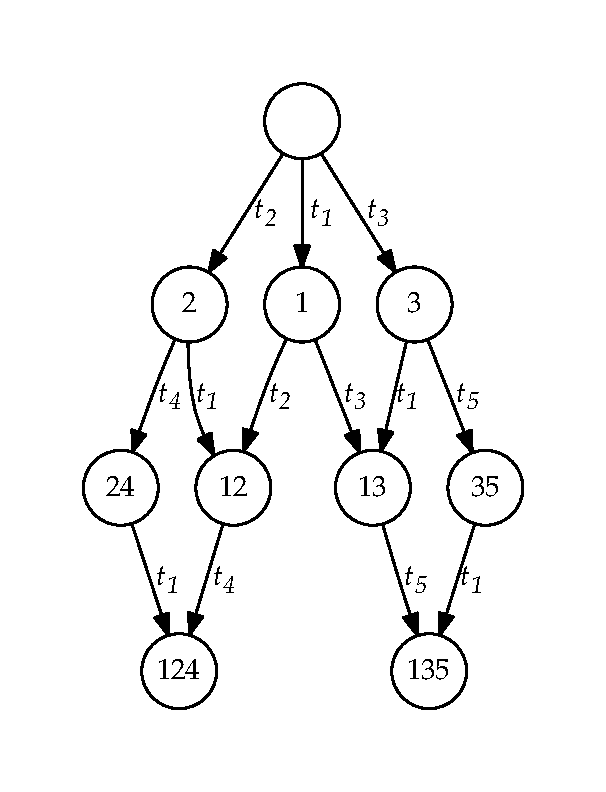
\includegraphics[height=9cm]{persistent1}
	\caption{Diagram of an example state space, for
		the illustration of persistent sets.}
	\label{fig:persistent}
\end{figure}

\subsubsection{Soundness}
Indeed, it can be shown that if a stopped state is reachable by an exhaustive
search of the state space, then by computing a persistent set $T$ at
each state $\sigma$ and exploring only those transitions from
$\sigma$ that are in $T$, that stopped state is still reachable
(cf. Theorem 4.3 in \textbf{Godefroid thesis}). It can also be shown
that by exploring only transitions in persistent sets, all reachable
local states of each process are explored (cf. Theorem 6.14 in
\textbf{Godefroid thesis}). Therefore, if we are interested in
the definition of model checking given in 
section~\ref{sec:simple-model-checking}, then it is sufficient
to explore transitions from the persistent sets of the states we
encounter.

\subsection{Sleep Sets}

Another technique for addressing the state explosion
problem is that of \emph{sleep sets}. Suppose that
we are at state $\sigma_0$ when performing a search
of the state space (see figure~\ref{fig:sleep}).
Suppose that the first transition
we explore is $t_1$, reaching $\sigma_1$,
and the second is $t_2$, reaching $\sigma_2$.
If $t_1$ and $t_2$ are independent, then there
is a state $\sigma'$ reachable by both
$\sigma \xrightarrow{t_1} \sigma_1
\xrightarrow{t_2} \sigma'$ and
$\sigma \xrightarrow{t_2} \sigma_2
\xrightarrow{t_1} \sigma'$.
Any stopped state reachable from $\sigma'$
is reachable from $\sigma_1$, as $\sigma_1$
is reachable from $\sigma'$. By assumption,
when the search is at $\sigma_2$, we have already
explored all the stopped states reachable from
$\sigma_1$ (the dotted area in figure~\ref{fig:sleep}),
in particular those reachable from
$\sigma'$. Therefore, there is no need to
explore $t_1$ from $\sigma_2$.

In fact, there is no need to consider executing
$t_1$ in our recursive exploration from $\sigma_2$
until we execute some transition $t'$ which is
\emph{not} independent of $t_1$, as after
the execution of $t'$, exploring $t_1$ may
now lead to an unexplored area of the state space.

A \emph{sleep set} for a particular state
is then the set of transitions which, when
explored, is guaranteed by the above
argument to lead to an already-explored
section of the state space\footnotemark.
\footnotetext{In the literature, sleep
	sets seem to be defined as the sets used
	in the sleep set algorithm, so a
	better definition cannot be given here.}
The technique of
sleep sets is orthogonal to the technique
of persistent sets -- there is no interaction
between the two techniques, so implementing
both simultaneously can be achieved with
no extra difficulty.

\begin{figure}
	\centering
	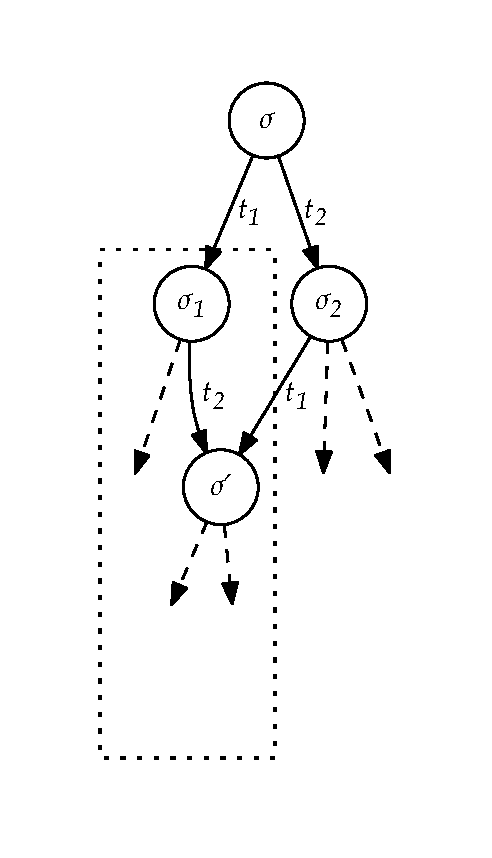
\includegraphics[height=8cm]{sleep}
	\caption{Diagram illustrating of the theory
		of sleep sets.}
	\label{fig:sleep}
\end{figure}

\section{Dynamic Partial-Order Reduction}
\label{sec:dpor-prep}
After reading this section, you should
understand how the dynamic
partial-order reduction algorithm works.

\subsection{Background Definitions}
The DPOR makes use of several new concepts,
which are presented here.

\subsubsection{Transition Sequences}
Instead of keeping track of just the current state, as
the algorithms in section~\ref{sec:simple-model-checking}
did, the DPOR algorithm keeps track of a \emph{transition
sequence} $\pi \in \mathcal{T}^*$. This transition
sequence is implicitly executed from the initial state of
the transition system, $\sigma_0$, so that in practice,
$\pi = t_0, t_1, \ldots, t_{n-1}$ determines a sequence of states
$\sigma_0, \sigma_1, \ldots, \sigma_n$ such that
\[
	\sigma_0 \xrightarrow{\ t_0\ } \sigma_1 \xrightarrow{\ t_1\ }
	\ldots \xrightarrow{t_{n-1}} \sigma_n.
\]

Given a transition sequence $\pi = t_0, t_1, \ldots, t_{n-1}$,
we use the following notation:
\begin{itemize}[label={}]
	\newcommand{\defsindent}{3.5em}
	\item{\makebox[\defsindent]{\hfill$\pi_i$}
		--- the transition $t_i$;}
	\item{\makebox[\defsindent]{\hfill$\pi.t$}
		--- the transition sequence $\pi$ extended with
		an additional transition $t$;}
	\item{\makebox[\defsindent]{\hfill$\textit{dom}(\pi)$}
		--- the set $\{i \in \mathbb{N} \mid 0 \leq i < n \}$;}
	\item{\makebox[\defsindent]{\hfill$\textit{pre}(\pi, i)$}
		--- the state $\sigma_i$ (i.e. the
		state immediately before transition $t_i$); and}
	\item{\makebox[\defsindent]{\hfill$\textit{last}(\pi)$}
		--- the final state, $\sigma_n$.}
\end{itemize}

\subsubsection{The Happens-Before Relations}\label{sec:happens-before}

Suppose that two adjacent transitions, $\pi_i$ and $\pi_{i+1}$,
are swapped in a
transition sequence, $\pi$, to give a new
transition sequence, $\pi'$. Suppose further
that $\pi_i$ and $\pi_{i+1}$ are independent.
Since $\pi_{i+1}$ is enabled in $\textit{pre}(\pi, i+1)$,
$\pi_{i+1}$ must also be enabled in $\textit{pre}(\pi, i)$,
as independent transitions cannot disable one another.
If $\pi_{i+1}$
is executed in $\textit{pre}(\pi, i)$,
it results in a state in which $\pi_i$
can be executed, as it cannot be disabled by $\pi_{i+1}$.

Because independent transitions commute, the state reached by
executing $\pi_i$ followed by $\pi_{i+1}$ is the same
as the state reached by executing $\pi_{i+1}$ followed
by $\pi_i$.
So $\textit{pre}(\pi, i+2) = \textit{pre}(\pi', i+2)$. Since 
for all $j \geq i + 2$, $\pi_j = \pi'_j$, it follows that
$\textit{last}(\pi) = \textit{last}(\pi')$. So swapping
a pair of adjacent transitions results in the same
final state if the transitions are independent.

\begin{figure}
	\centering
	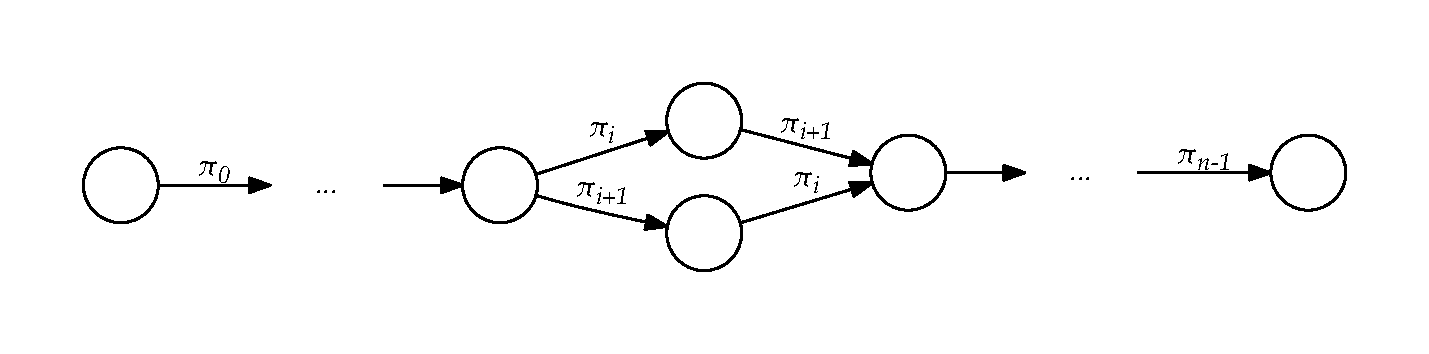
\includegraphics[width=\textwidth]{seqequiv}
	\caption{Illustration}
	\label{fig:sequence-equivalence}
\end{figure}

Such equivalent interleavings
of transitions are precisely what we are interested in.
We can think of a transition sequence as representing
the equivalence class of transition sequences obtained
by swapping adjacent pairs of independent transitions;
if we can identify that two transition sequences are
members of the same equivalence class, we need only
explore one.

To help us to reason about such equivalence classes,
we will use a ``happens-before" relation to identify
when one transition cannot be swapped with another.
In particular, we define the \emph{happens-before}
relation $\longrightarrow_\pi$ for a transition
sequence $\pi$ to be the smallest relation on
$\textit{dom}(\pi)$ such that
\begin{enumerate}
	\item if $i \leq j$ and $\pi_i$ is dependent with
		$\pi_j$ then $i \longrightarrow_\pi j$; and
	\item $\longrightarrow_\pi$ is transitively closed.
\end{enumerate}

By construction, the happens-before relation is a
partial-order relation on the transitions in $\pi$,
and $\pi$ is one of the linearisations of this
partial order. The other linearisations of the
partial order are the equivalent sequences of
transitions which can be obtained by swapping
adjacent pairs of independent transitions in $\pi$.

The DPOR algorithm also makes use of a variant of the
happens-before relation.
Informally, if $(i, p)\!\hookrightarrow_\pi$ then
in every linearisation $\hat{\pi}$ of the
happens-before relation (that is, every sequence
obtained by swapping pairs of adjacent,
independent transitions in $\pi$), the next
transition that process $p$ executes in
state $\textit{pre}(\pi, i)$ is executed
at some point before $\textit{last}(\hat{\pi})$.
Formally, 
if $i \in \textit{dom}(\pi)$ and $p \in
\mathcal{P}$ then we
say that $(i, p)\!\hookrightarrow_\pi$ if
either
\begin{enumerate}
	\item $\textit{proc}(\pi_i) = p$; or
	\item $\exists k \in \textit{dom}(\pi).\;
	i < k \,\wedge\, \textit{proc}(\pi_k) = p
	\,\wedge\, i \longrightarrow_\pi k $.
\end{enumerate}


\subsection{The DPOR Algorithm}

\subsubsection{Overview}

The Dynamic Partial-Order Reduction (DPOR) algorithm
dynamically uses information gathered during its
exploration of a search space to explore only
transitions in a persistent set from each state
encountered on the search -- a partial-order
reduction technique. The idea is that the
extra information which is available because
the persistent sets are created dynamically
allows smaller (and therefore more efficient)
persistent sets to be chosen than an algorithm
computing its persistent sets statically.

In particular, at each state $\sigma$, the
next transition
to execute, $t$, is chosen at random, and it is
initially assumed that that transition will
be the only transition to be explored from
that state. However, this is a persistent
set only if $t$ is
independent of every transition reachable
by exploring any transitions
from $\sigma$ other than $t$. Clearly,
this isn't true in general, so, at each
state $\sigma'$ encountered beyond
$\sigma$, if there is a transition
$t' \in \textit{enabled}(\sigma')$
such that $t'$ is dependent with
$t$ and $t'$ may appear before $t$
in an exploration from $\sigma$, then
a backtracking point is added at
$\sigma$ to ensure that such an
exploration is made. Over time,
the addition of such backtracking points
ensures that the set of transitions
explored from each state is a
persistent set.


\newcommand{\dporpseudocode}{
	\begin{algorithmic}[1]
		\Procedure{Explore}{$\pi$}
		\Let{$\sigma$}{$\textit{last}(\pi)$}
		\ForAll{$p \in \mathcal{P}$}
		\State \Call{UpdateBacktrackSets}
		{$\pi,\, \textit{next}(\sigma, p)$}
		\EndFor
		\If{$\textit{enabled}(\sigma) \neq \emptyset$}
		\Let{$t$}{any $t \in \textit{enabled}(\sigma)$}
		\Let{$\textit{backtrack}(\sigma)$}{$\{t\}$}
		\Let{$\textit{done}(\sigma)$}{$\emptyset$}
		\While{$\textit{done}(\sigma)
			 \neq \textit{backtrack}(\sigma)$}
		\Let{$t$}{any $t \in (\textit{backtrack}(\sigma)
			\setminus \textit{done}(\sigma))$}
		\State add $t$ to $\textit{done}(\sigma);$
		\State \Call{Explore}{$\pi.t$}

		\EndWhile
		\EndIf
		\EndProcedure
		\State
		\Procedure{UpdateBacktrackSets}{$\pi,\, t_{p,s}$}
		\Let{$D$}{$\{i \in \textit{dom}(\pi) \mid
			\pi_i \text{ is dependent with } t_{p,s}
			\text{ and } (i, p)\!\not \hookrightarrow_\pi \}$}
		\If{$D \neq \emptyset$}
		\Let{$\sigma_d$}
		{$\textit{pre}(\pi,\text{max}(D))$}
		\If{$\textit{next}(\sigma_d, p)
			\in \textit{enabled}(\sigma_d)$}
		add $\textit{next}(\sigma_d, p)$
		to $\textit{backtrack}(\sigma_d)$
		\Else {
			add all of $\textit{enabled}(\sigma_d)$
			to $\textit{backtrack}(\sigma_d)$
		} \EndIf
		\EndIf
		\EndProcedure
		\State
		\State Initially: \Call{Explore}{$\emptyset$}
	\end{algorithmic}
}
\begin{figure}
	\dporpseudocode
	\caption{The DPOR algorithm}
	\label{dpor-outline} 
\end{figure}

\subsubsection{Line-By-Line Explanation}
\label{sec:dpor-prep-walkthrough}
\begin{description}
	\item[Lines 1--2] The \textsc{Explore} procedure implements
	dynamic partial-order reduction. The transition sequence
	$\pi$ which is passed as its argument specifies the state
	from which the exploration is to take place, $\sigma$.

	\item[Lines 3--4] First, any necessary backtracking points
	which can be identified from this state are added to the
	\textit{backtrack} sets of previous states. Backtracking
	points can be identified using information from each possible
	transition from this state, so the \textsc{UpdateBacktrackSets}
	procedure is called with each possible next transition as an
	argument.

	\item[Line 5] Having updated the \textit{backtrack} sets
	of previous states, the search continues its exploration,
	but only if there are any enabled transitions to explore.

	\item[Lines 6--8] The recursive exploration proceeds by
	maintaining two sets of transitions: \textit{backtrack}
	and \textit{done}. The \textit{backtrack} set contains
	those transitions from $\sigma$ which should be explored,
	and is initialised to any enabled transition. Recursive calls to
	\textsc{Explore} may add more transitions to \textit{backtrack}.
	The \textit{done} set contains those transitions
	in \textit{backtrack} that have been explored.

	\item[Line 9] The search from $\sigma$ halts when every
	transition that needs to be explored (is in \textit{backtrack})
	has been explored (is in \textit{done}).

	\item[Lines 10--12] If there is some transition that needs
	exploring, \textsc{Explore} is recursively called with that
	transition extending the current transition sequence $\pi$,
	that transition is added to \textit{done}.

	\item[Line 14] The \textsc{UpdateBacktrackSets} procedure
	can use the information that a given transition, $t_{p,s}$ can be
	executed in $\sigma$ to add necessary backtracking points.

	\item[Line 15] The set $D$ contains the indices $i$ of the
	transitions $\pi_i$ in the sequence such that $\pi_i$ and
	$t$ are dependent, and $(i, p)\!\not \hookrightarrow_\pi$.
	This second condition means that $t_{p,s}$ is \emph{not}
	guaranteed to happen after $\pi_i$, so $D$ is the set
	of transitions which may have a race condition with
	$t_{p,s}$.

	\item[Line 16] If there are no transitions which have
	a race condition with $t_{p,s}$, then no backtracking
	points need to be added: as far as we know from $t_{p,s}$,
	if we had chosen any other
	choices of transitions to explore previously, we would
	have ended up with a transition sequence in the same
	equivalence class as $\pi$.

	\item[Line 17] If there are transitions in $\pi$
	which have a race condition with $t_{p,s}$, then
	it is sufficient to add a backtracking point at
	the state immediately before
	the most recent of these;
	the necessary backtracking
	points for the earlier states will be added
	by later (or previous) calls of \textsc{Explore}.

	\item[Line 18] We know there is a race condition
	between $t_{p,s}$ and $\textit{next}(\sigma_d,p)$, so
	we want to explore another transition sequence from
	$\sigma_d$ in which $\textit{next}(\sigma_d,p)$
	appears before $t_{p,s}$. If $\textit{next}(\sigma_d,p)$
	is enabled in $\sigma_d$, then we certainly explore such
	a transition sequence by immediately exploring
	$\textit{next}(\sigma_d,p)$ from $\sigma_d$.

	\item[Line 19] However, if we cannot immediately
	explore $\textit{next}(\sigma_d,p)$
	from $\sigma_d$ because it is not enabled, then it is
	not obvious which transitions to explore from $\sigma_d$
	 to achieve
	a transition sequence in which $\textit{next}(\sigma_d,p)$
	appears before $t_{p,s}$. The algorithm presented here
	does not attempt to narrow down which transitions might
	lead to such a transition sequence, and instead plays it
	safe and explores them all.

	\item[Lines 21] To perform model checking, the state space
	is explored from the initial state, $\sigma_0$, which is
	reached from $\sigma_0$ by executing no transitions, so
	\textsc{Explore} is initially called on the empty
	sequence of transitions, $\emptyset$.

\end{description}

\subsubsection{Example Execution}
An example execution, on the same example as
figure~\ref{fig:sdpor-motivation}.

\section{Summary}
Having read this chapter,
you should now understand:
\begin{understandinglist}
	\item what a process, state, transition
	and transition system are;
	\item that model checking in the
	context of my project is the process
	of deciding whether a given transition
	system is both error-free and deadlock-free
	by exploring possible executions of the
	system;
	\item that a simple model checking algorithm
	performs an exhaustive depth-first search
	of the state space, checking for errors and
	deadlocks at each state encountered;
	\item that persistent sets use information
	about the independence of transitions to
	avoid exploring sections of the state space
	which are equivalent to sections that \emph{are}
	explored;
	\item that sleep sets use information about
	the independence of transitions and the history
	of the search of the state space to avoid
	exploring a section of the state space which
	has already been explored;
	\item that the dynamic partial-order
	reduction algorithm executes one arbitrary
	and full interleaving of the concurrent program,
	then uses information about independence and
	which transitions happen-before others to
	add backtracking points, so that a
	persistent set is explored from each state; and
	\item that most of my work before implementing
	the project was reading and understanding theory,
	but I also planned how I would approach the
	implementation.
\end{understandinglist}

\chapter{Implementation}
After reading this chapter,
you should understand:
\begin{understandinglist}
	\item the high-level structure and
	organisation of my project;
	\item the software development approach
	I used in developing the project;
	\item the decisions I made
	when designing and implementing
	the programming language used
	as the object language for the
	project; and
	\item the details of my
	implementations of the
	algorithms in the project.
\end{understandinglist}

\section{Design of the Software}
After reading this section, you
should understand the high-level
design decisions I made in the
development of the project, and
the reasoning behind them.
\bigskip

\noindent
The project was implemented in OCaml, which
offers a few key advantages:
\begin{itemize}
	\item a clean, functional
	style, which is particularly appropriate for
	this project, given its mathematical nature;
	\item a strong, safe type system, which makes
	impossible a large class of runtime errors;
	\item parametric polymorphism, a module system,
	and other higher-order programming features,
	facilitating abstraction and generalisation; and
	\item established libraries, providing efficient
	implementations of basic data structures and algorithms.
\end{itemize}
I took particular advantage of the module system when
designing and implementing the project. OCaml modules
are used to encapsulate related definitions and hide
information -- \emph{signatures} are software interfaces
providing declarations,
and \emph{structures} are implementations which 
provide definitions. A structure \emph{matches} a
signature if it has a definition for each declaration
in the signature. \emph{Functors} can be thought of
as functions from structures to structures. If a
module matches a given signatures, then it can be
passed to a functor to give a new structure.

\begin{figure}
	\centering
	\begin{subfigure}{.4\textwidth}
		\centering
		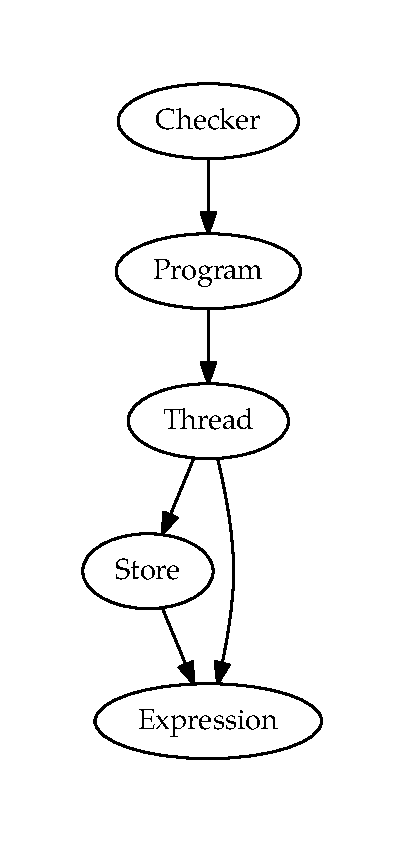
\includegraphics[height=9cm]{interfaces}
		\caption{Diagram showing which signatures declare
			which other signatures as nested sub-structures.}
		\label{fig:interfaces}
	\end{subfigure}%
	\quad
	\begin{subfigure}{.5\textwidth}
		\centering
		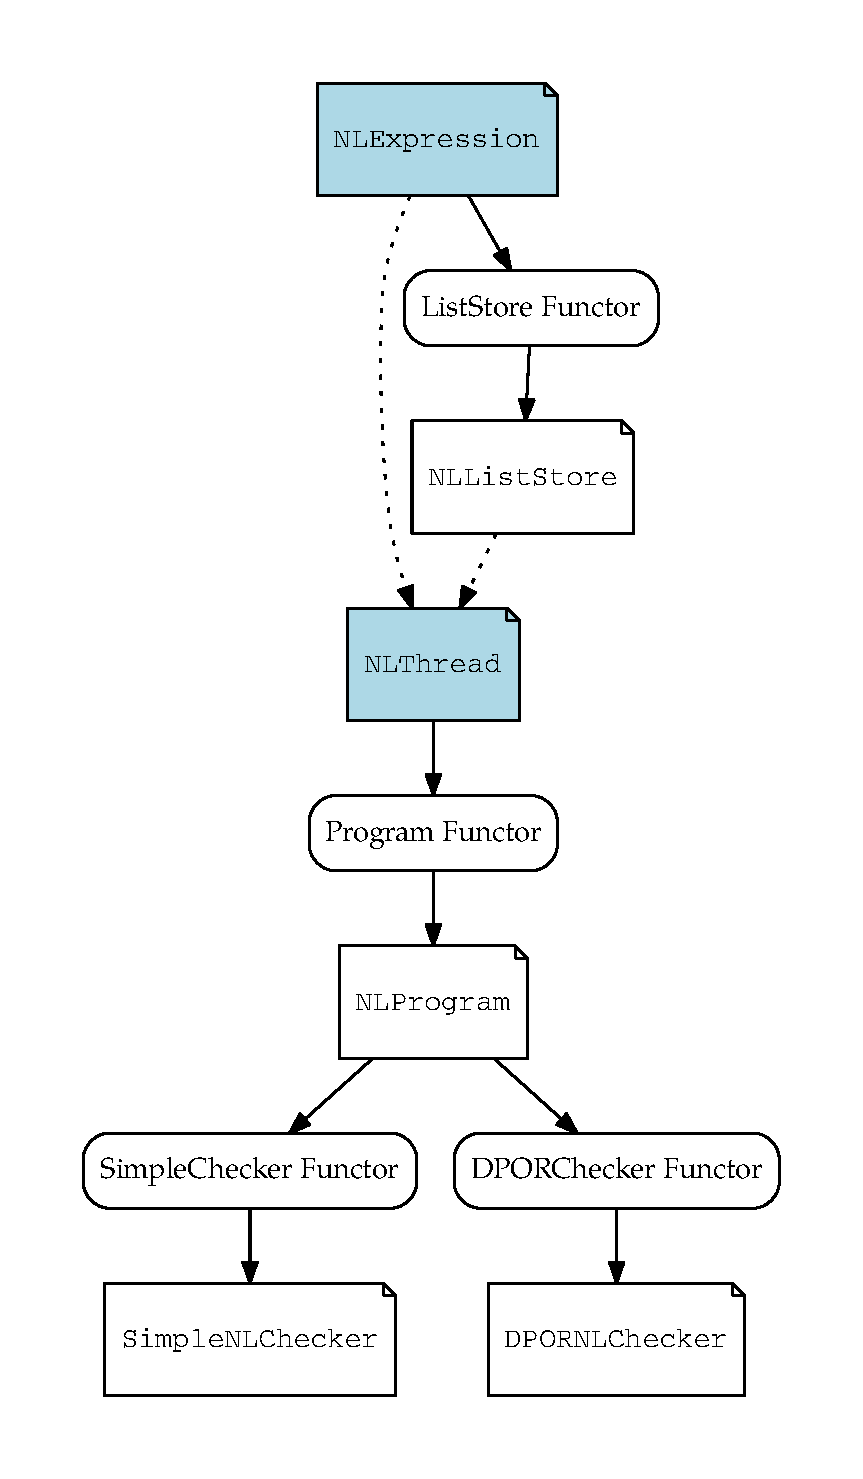
\includegraphics[height=12cm]{functors}
		\caption{Diagram showing generation of
			structures using functors. The blue files must be provided;
			the functors are part of this project; the remaining files
			are generated using the functors.}
		\label{fig:functors}
	\end{subfigure}
	\caption{Diagrams showing the interactions between
		the software modules.}
	\label{fig:design}
\end{figure}

In the project, there are five main signatures:
\begin{enumerate}
	\item a structure that matches \emph{Expression}
	contains information about the structure of expressions
	in the programming language of interest;
	\item a structure that matches \emph{Store}
	implements a store (i.e. a mapping from locations
	to expressions) for some implementation of \emph{Expression};
	\item a structure that matches \emph{Thread} contains
	the information about the semantics of expressions
	for a programming language;
	\item a structure that matches \emph{Program}
	contains declarations relating to
	transition systems as expressed in some programming
	language; and
	\item a structure that matches \emph{Checker}
	contains a function which performs model checking.
\end{enumerate}

While I did implement a simple programming language
(see section~\ref{sec:language}), the model checking
algorithms that are the focus of this project are of
course entirely independent of any particular language.
I therefore ensured that, in order to use
my project to perform model checking for programs
in any other language, the work that would have to
be done would be minimal. In particular, given implementations
of \emph{Expression} and \emph{Thread} (effectively
specifying the semantics of a programming language), my system uses
functors to automatically generate implementations of
\emph{Store}, \emph{Program} and \emph{Checker}, the
last of which can then be used to immediately perform
model checking. This process is shown explicitly in
figure~\ref{fig:functors}.

\section{Development of Project Language}
\label{sec:language}
After reading this section, you should
understand the process of designing
and implementing the programming
language in which the programs to
be model checked are written,
including the reasoning behind
the decisions I made.

\subsection{Language Design}
\textbf{First, the language had to be designed.
	Explain design choices, give sense of what
	the language is, maybe an example program,
	and point to the appendix for a full definition.}

Although, as mentioned above, any programming language
could be used to express transition systems for model
checking, I chose to design and implement a simple
ML-like language, PL (Project Language), to avoid
the unnecessary complexity of implementing a full
industrial language.
The grammar for valid PL expressions is given in
figure~\ref{fig:pl-expressions}.

\begin{figure}
	\centering
	\setlength{\tabcolsep}{2pt}
	\begin{tabular}{rl}
		\textit{expr} $:=$ & \textit{int} $\vert$ \textit{bool} $\vert$ \textit{var} \\
		$\vert$ & \textit{local} $\vert$ \textit{global}
			$\vert$ \textit{spinlock} \\ 
		$\vert$ & \textit{expr op expr} $\vert$ $\neg\,$\textit{expr} \\
		$\vert$ & \textbf{skip} $\vert$ \textit{expr; expr}\\
		$\vert$ & \textbf{if} \textit{expr}
			\textbf{then} \textit{expr} \textbf{else} \textit{expr} \\
		$\vert$ & \textbf{while} \textit{expr}
			\textbf{do} \textit{expr} \\
		$\vert$ & \textit{expr} $:=$ \textit{expr} $\vert$ !\textit{expr} 
			$\vert$ \textbf{ref} \textit{expr} \\
		$\vert$ & \textbf{fn} \textit{var}
			$\Rightarrow$ \textit{expr} $\vert$ \textit{expr expr} \\
		$\vert$ & \textbf{let} \textit{var} $=$
			\textit{expr} \textbf{in} \textit{expr} \\
		$\vert$ & \textbf{let rec} \textit{var} $=$
			\textbf{fn} \textit{var} $\Rightarrow$
			\textit{expr} \textbf{in} \textit{expr} \\
		$\vert$ & \textbf{lock} \textit{expr} $\vert$
			\textbf{unlock} \textit{expr} \\
		$\vert$ & \textbf{cas}(\textit{expr}, \textit{expr}, \textit{expr}) \\
		$\vert$ & \textbf{error}(\textit{message}) \\
		& \\
		\textit{int} $\in$ & $\{\ldots, -1, 0, 1, \ldots\}$ \\
		\textit{bool} $\in$ & $\{\textbf{true}, \textbf{false}\}$ \\
		\textit{var} $\in$ & \textit{Variable}
	\end{tabular}
	\qquad\quad
	\begin{tabular}{rcl}
		\textit{op} $:=$ & $+$ &\\
		$\vert$ & $-$ &\\
		$\vert$ & $\ast$ &\\
		$\vert$ & $/$ &\\
		$\vert$ & $\%$ &\\
		$\vert$ & $>$ &\\
		$\vert$ & $<$ &\\
		$\vert$ & $=$ &\\
		$\vert$ & $\&$ &\\
		$\vert$ & $\mid$ &\\
		& &\\
		\textit{local} & $\in$ & \textit{Location} \\
		\textit{global} & $\in$ & \textit{Location} \\
		\textit{spinlock} & $\in$ & \textit{Location} \\
		& &\\
		\textit{Location} & $=$ & $\{a, b, c, \ldots\}^\ast$\\
		\textit{Variable} & $=$& $\{x, y, z, \ldots\}$ \\
	\end{tabular}
	\caption{The grammar for PL expressions.}
	\label{fig:pl-expressions}
\end{figure}

As required by the \emph{Thread} interface, each
PL thread has access to both its local store $s$
and the global store $g$. Both $s$ and $g$ are
maps from locations to expressions.
To express the semantics
of PL, then, we need to give whether or not an
expression $e$ reduces for local store $s$ and
global store $g$, and if it does, we need to give
the expression $e'$ that it reduces to in one ``step",
as well as any updates to $s$ and $g$ that result.
Note that each such ``step" is assumed to be atomic.
The semantics of PL expressions are as you would expect
(see \textbf{THE APPENDIX} for a full definition), but
the rules for the reduction of expressions that interact
with the global store $g$ are given in figure~\ref{fig:pl-rules}.

\begin{figure}
	\begin{gather*}
		\frac{g(\textit{spin}) = \textbf{true}}
			{(\textbf{unlock}\ \textit{spin},\ s,\ g)
				\longrightarrow (\textbf{skip},\ s,\
				g[\textit{spin} \mapsto \textbf{false}])} \\
		\\
		\frac{g(\textit{spin}) = \textbf{false}}
		{(\textbf{lock}\ \textit{spin},\ s,\ g)
			\longrightarrow (\textbf{skip},\ s,\
			g[\textit{spin} \mapsto \textbf{true}])} \\
		\\
		\frac{g(\textit{glob}) = e_\textit{curr}}
			 {(\textbf{cas}(\textit{glob},\, e_\textit{curr},\, e_\textit{new})
			 	,\ s,\ g) \longrightarrow (\textbf{true},\ s,
			 	\ g[\textit{glob} \mapsto e_\textit{new}])} \\
		\\
		\frac{g(\textit{glob}) \neq e_\textit{curr}}
			{(\textbf{cas}(\textit{glob},\, e_\textit{curr},\, e_\textit{new})
				,\ s,\ g) \longrightarrow
				(\textbf{false},\ s,\ g)} 
	\end{gather*}
	\caption{Rules for the atomic reduction of PL
		expressions that interact with the shared store.}
	\label{fig:pl-rules}
\end{figure}

There is no type system for PL. Although it would have been
beneficial to design and implement a type system for PL
(a type checker could catch type errors early, rather than a runtime
failure with non-obvious causes occurring), I thought that the total
time I would have spent on creating the type system would be more than
the time taken in dealing with the problems resulting from having
no type system. With the benefit of hindsight, I think this was the
correct decision.

\subsection{Parser}
On the other hand, I decided that investing time in creating a
parser for PL would pay itself off over the course of the project.
This allows me to write, for example,
\begin{align*}
	\texttt{let y = ref 1 in cas(Gx, 7 * !y - 3, 0)},
\end{align*}
instead of having to type the OCaml meta-language abstract
syntax tree representing the structure of the Pl expression:
\begin{align*}
	\texttt{Let (Ref (Integer}& \texttt{ 1), Cas (Global "x",
		Op (Op (Integer 7,} \\ \texttt{Mult,}& \texttt{ Deref (Var 0)), Minus, Integer 3),
		Integer 0))}.
\end{align*}
Writing such expressions is not only extremely time-consuming but
also error-prone. For the language to be of any practical use,
a parser is a necessity.

To create a parser for PL, two program generators were used:
\emph{OCamllex} and \emph{Menhir}. When presented with a
file giving a mapping from strings of characters to tokens,
OCamllex produces a lexical analyser, which converts a sequence
of characters into a sequence of tokens. When presented with a
grammar and a set of precedence rules, Menhir produces a parser,
which converts a sequence of tokens into an abstract syntax tree
of the grammar. These were used in conjunction, as shown in
figure~\ref{fig:parsing}, to produce a PL parser.

\begin{figure}
	\centering
	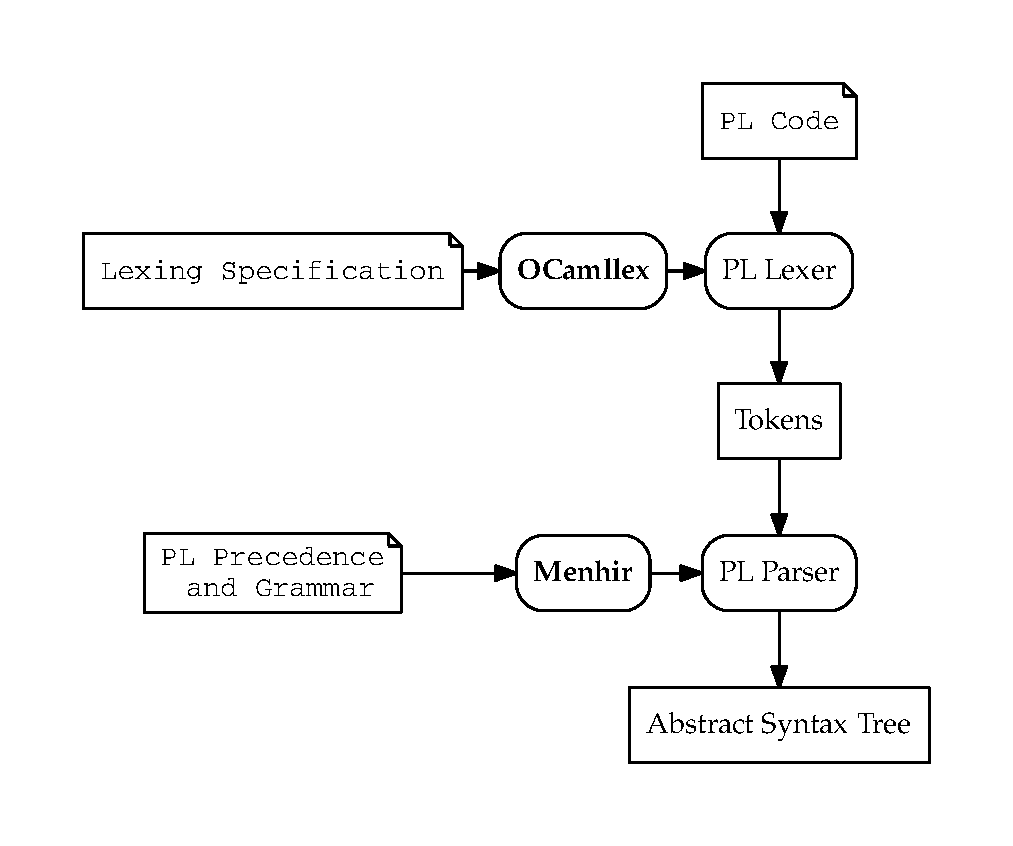
\includegraphics[height=10cm]{parsing}
	\caption{Diagram showing the flow and processing of
		information in the generation of a PL abstract
		syntax tree.}
	\label{fig:parsing}
\end{figure}

\subsection{Implementation}

\subsubsection{The Expression Module}
There are actually two datatypes which are used to
represent PL expressions in the
PL implementation of the \emph{Expression} module.
The first of these is the ``raw" expression, which
uses strings to represent variables (this is the
datatype that the parser produces). However,
manipulation of expressions is much easier when
variables are represented using \emph{de Bruijn indices},
which is the purpose of the second expression datatype.
This is the only one required by the \emph{Expression}
signature. A function exists to recursively convert
from the ``raw" datatype to this second datatype.

The remainder of the \emph{Expression} module
consists of auxiliary functions, which are
necessary for the implementation of later
modules, and either return a simple piece
of information or perform a simple manipulation.

\subsubsection{The Store Module}
As mentioned above, I implemented a functor
called \textbf{ListStore}, which, given a structure
matching the \emph{Expression} signature,
gives a structure matching the \emph{Store}
signature. The \emph{Store} implementation produced
represents stores using a simple list of
(location, expression) pairs. If a location
appears twice in the list, the occurrence
nearest the head of the list is taken to be
the correct value. A function is provided
which walks through from head to tail and
removes any stale pairs, which although
linear in time, reduces the space taken
by the list.

More efficient store implementations are of
course possible (for example, one based on
a hash table rather than a list), but
I went for the simplest reasonable
implementation I could think of, to
ensure correctness.

The only other function of note is
\texttt{get\_fresh\_loc},
which queries the \emph{Expression} \texttt{random\_loc}
function until it returns a result which is
unbound in the store. This is used to generate a location
to use when a new local reference is created using the
\textbf{ref} keyword.

\subsubsection{The Thread Module}
The \emph{Thread} module consists mostly of
the \texttt{next\_step} and \texttt{next\_transition}
functions. The \texttt{next\_step} function uses pattern
matching on PL expressions to determine what the next atomic
operation, if any, to be executed in the reduction
of the expression is. There is a close correspondence
between the
rules of the operational semantics (see \textbf{APPENDIX})
and the different cases in the pattern matching. This is
because each rule specifies that an expression of a
particular form, perhaps with some conditions on the
states of the local and shared stores, reduces in a
particular way. For illustration, one rule and its
corresponding pattern matching case is shown in 
figure~\ref{fig:step-rule-correspondence}.

\begin{figure}
	\begin{subfigure}{\textwidth}
		\begin{gather*}
		\frac{}
		{(\textbf{if true then } e_2 \textbf{ else }
				e_3,\,s,\,g) \rightarrow (e_2,\,s,\,g)}
		\qquad
		\frac{}
		{(\textbf{if false then } e_2 \textbf{ else }
			e_3,\,s,\,g) \rightarrow (e_3,\,s,\,g)} \\
		\\
		\frac{(e_1,\,s,\,g) \rightarrow
			(e_1^{\prime},\,s^{\prime},\,g^{\prime})}
		{(\textbf{if } e_1 \textbf{ then }
			e_2 \textbf{ else } e_3,\,s,\,g)
			\rightarrow (\textbf{if } e_1^{\prime}
			 \textbf{ then }
			e_2 \textbf{ else } e_3,\,
			s^{\prime},\,g^{\prime})}
		\end{gather*}
		\caption{Rules relating to
			the reduction of if-then-else expressions.}
	\end{subfigure}
	\\ \\ \\
	\begin{subfigure}{\textwidth}
		\lstinputlisting[frame=none, firstline=59, lastline=63]
			{../src/pl_thread.ml}
		\caption{Pattern matching case for if-then-else expressions.
			If \texttt{e1} is a Boolean, then reduce to \texttt{e2} or
			\texttt{e3},
			otherwise use a recursive call to try to reduce \texttt{e1}.}
	\end{subfigure}
	\caption{A concrete illustration of the correspondence
		between the rules of the operational semantics
		and the pattern matching statements of the
		\texttt{next\_step} function.}
	\label{fig:step-rule-correspondence}
\end{figure}

As a transition for a thread is defined as a
finite sequence of \emph{invisible} local
operations, followed by one \emph{visible} operation
which accesses the shared store, the \texttt{next\_transition}
function simply repeatedly calls the \texttt{next\_step}
function, reducing the initial expression and modifying
the local store, until either the resulting step accesses the shared
store, or no further reduction is possible. Noting that this
process is independent of the object language (PL, in this case),
the most general implementation of this project would require
only the  \texttt{next\_step} function to be provided by
the user, with a functor being used to automatically
produce the \texttt{next\_transition} function. However,
in this case, I decided that the additional design complexity
cost was not worth the slight improvement to the abstraction
of the project.

\subsubsection{The Program Module}
The \emph{Program} module is a small functor which,
when given a \emph{Thread} implementation, provides 
the few additional definitions and auxiliary
functions necessary to fully represent
transition systems (cf. section~\ref{sec:background-defs}.)
In particular, a state $\sigma \in \textit{State}$ is
represented by an instance of the \texttt{state} type:
\lstinputlisting[frame=none, firstline=107, lastline=107]
	{../src/interfaces.ml}

\subsubsection{Testing}
To ensure that the implementation of the PL
language was correct, I wrote unit tests for
the \texttt{next\_transition} and
\texttt{next\_step} functions. These tests
consisted of a series of inputs and expected outputs
to these functions. My aim in writing these tests
was to ensure that most of the code was covered,
so that any obvious bugs could be corrected
immediately. However, I did not invest time
making these tests very rigorous for two reasons:
any bugs found later would be relatively straightforward
to correct, and getting the PL implementation
fully correct was not the aim of the project, but
just a necessary step before the main work on the
model checking algorithms.

\section{Simple Model Checker}
After reading this section, you
should understand how I implemented
the simple model-checking algorithm,
particularly how the results (whether
a given state is error-free and
deadlock-free) are computed,
and also how this implementation
was tested.

In order to ensure the correctness of my implementation
of the DPOR algorithm, to have a baseline to use
for performance comparison, and to begin by implementing
a relatively simple model checking algorithm, I first wrote the
SimpleChecker functor, which takes an implementation of
\emph{Program} as its input, and outputs a structure
which provides
a function that performs model checking by performing
an exhaustive depth-first search of the state space --
the simplest possible model checking algorithm.

\subsection{Implementation}
\label{sec:simple-imp}

See the \textbf{APPENDIX} for an illustration
of the relationship between the actual OCaml
code, and the pseudocode given in
figure~\ref{fig:simple-imp-code}, which gives
a high-level description of the algorithm,
which performs an exhaustive depth-first
search of the state space as outlined in
section~\ref{sec:simple-model-checking},
deciding at each state whether the state space
from the current state onwards is error-free
and deadlock-free.

\subsubsection{Detecting Errors}

The algorithm assumes that if a thread
encounters an error, then the execution
of that thread will not proceed, meaning
that only threads which do not have an
enabled next transition need to be checked
for errors. The Boolean \textit{error\_free}
tracks whether any threads in the current state
have encountered an error (line 14) and whether any
recursive calls report an error (line 11), and is
returned as one of the two Boolean results
of the call (line 17).

\subsubsection{Detecting Deadlocks}

Deciding whether the state space from the current
state onwards is deadlock-free is more complicated.
The \textit{calls\_deadlock\_free} keeps track of
whether any recursive call reports a deadlock. If
any do, then it is set to false (line 12), causing the
algorithm to report that the state space herein
is not deadlock-free (line 17).

Assuming that no
recursive calls report a deadlock, then the state
space is deadlock-free if and only if the current
state is not a deadlock state, which is the case
if and only if either there is some thread with an
enabled transition,
or every thread had terminated its computation and
is not waiting for some change in the global state.
Two Booleans keep track of these two possibilities:
if any transition is enabled, then
\textit{is\_enabled\_thread} is set to true (line 9),
and if any thread without an enabled transition is
waiting for some change in the shared state (for
instance a lock to become available), then
\textit{no\_waiting\_threads} is set to false.
If either Boolean is true at the end of the call
to \textsc{Check}, then, providing no recursive
calls reported a deadlock, the algorithm returns
that the state space is deadlock-free.

\begin{figure}
	\begin{algorithmic}[1]
		\Procedure{Check}{$\sigma_0,\,\pi$}
		\Let{$(l, g)$}
			{$\textit{last}(\pi)$}
		\Let{\textit{error\_free}}{true}
		\Let{\textit{is\_enabled\_thread}}{false}
		\Let{\textit{no\_waiting\_threads}}{true}
		\Let{\textit{calls\_deadlock\_free}}{true}
		\ForAll{$p \in \mathcal{P}$}
		\If{$\textit{next}(\sigma, p) \in \textit{enabled}(\sigma)$}
			\State \textit{is\_enabled\_thread} := true;
			\Let{$(\textit{result\_ef}, \textit{result\_df})$}
				{\Call{Check}{$\sigma_0, \pi.\textit{next}(\sigma, p)$}}
			\State \textit{error\_free} := \textit{error\_free}
				\& \textit{result\_ef};
			\State \textit{calls\_deadlock\_free}
			:= \textit{calls\_deadlock\_free}
			\& \textit{result\_df}
		\Else
			\If{$\textit{err}(l(p))$}{ \textit{error\_free} := false};
			\EndIf
			\If{$\exists g' \in \mathcal{G}.\;
				\textit{next}(\sigma,p) \in \textit{enabled}(l,g')$}
				{\textit{no\_waiting\_threads} := false}
			\EndIf
		\EndIf
		\EndFor
		\Let{\textit{deadlock\_free}}{\textit{calls\_deadlock\_free} \&
			(\textit{is\_enabled\_thread} | \textit{no\_waiting\_threads})}
		\State \Return (\textit{error\_free}, \textit{deadlock\_free})
		\EndProcedure
	\end{algorithmic}
	\caption{Simple model checking algorithm}
	\label{fig:simple-imp-code}
\end{figure}

\subsection{Testing}

Although more detail will be given in
section~\ref{sec:pl-checker-tests}, it
is worth mentioning here that before going
on to implement anything else, I first
tested the simple model checker to weed
out any obvious bugs in either the
implementation of PL or of the simple
model checker itself; the bugs would need
dealing with at some point anyway, so
better to catch them as soon as possible,
when it would be easiest to identify the
causes.

Each simply gave a PL program,
ran the simple model checker on it, and
raised a flag if the result was not as
I expected. It wasn't difficult to
provide high code coverage of this
relatively simple algorithm. Along
with the simplicity of the algorithm,
these tests gave me confidence in
the correctness of my implementation.

\subsection{Correctness}

The reason that I have fully explained
the operation of this simple model checker,
provided a mapping
in the \textbf{APPENDIX} from the OCaml
implementation to the high-level
pseudocode, and described
tests of its correctness is to give the reader
as much confidence as possible
that the implementation performs
model checking as defined in
section~\ref{sec:model-checking-dfn}; in
chapter~\ref{cha:evaluation}, the
correctness of the simple model checker will be used
to provide evidence that the implementations of
other model checking algorithms are also correct.

\section{Dynamic Partial-Order Reduction}
The Dynamic Partial-Order Reduction (DPOR)
algorithm was presented in section~\ref{sec:dpor-prep},
which gave an overview of its operation,
including high-level pseudocode, reproduced
in figure~\ref{fig:dpor-imp-pscode} for ease
of reference. Several
aspects of the algorithm mean that it
is not obvious how it can be implemented
as an executable program; after reading
this section, you should understand
how this was achieved.

\begin{figure}
	\dporpseudocode
	\caption{The DPOR pseudocode}
	\label{fig:dpor-imp-pscode}
\end{figure}

\subsection{Implementation}
Section~\ref{sec:dpor-prep-walkthrough} gave a
line-by-line explanation of how
the DPOR algorithm works. This section gives a
line-by-line explanation of how the algorithm
was implemented.

\begin{description}
	\item[Line 1] The \textsc{Explore} procedure
	is implemented as a recursive OCaml function,
	\texttt{check}.
	One of the advantages of OCaml is its provision
	of practical procedural features, as well the
	functional ML features, which usefully allowed
	me to combine these styles as I saw fit when
	implementing this algorithm.

	\item[Line 2] When implementing the simple
	model checker, I used the \texttt{fold\_left}
	function from the provided List module to
	repeatedly use the \texttt{apply\_transition}
	from the \textit{Program} module to apply
	the transitions in the transition sequence
	to the initial state. However, in this case
	I wrote a function, \texttt{pre},
	which applies only the first
	$n$ transitions in the sequence,
	thereby returning the state
	$\textit{pre}(\pi, n)$ if $n < |\pi|$
	or the state $\textit{last}(\pi)$ if
	$n = |\pi|$, which is what we want in
	this case.

	\item[Lines 3--4] The \texttt{next\_transition}
	function, provided in the \textit{Thread} module,
	may return no transition at all (for instance
	in the case that a thread has terminated its
	computation), so the call to 
	\textsc{UpdateBacktrackSets} is only made if
	\texttt{next\_transition} does return a
	transition. It is also here, in the
	iteration through the threads,
	that it is decided whether the current
	state is an error or a deadlock
	(see section~\ref{sec:spor-imp-detecting}
	below).

	\item[Lines 15--17] In this project,
	the assumptions are made that
	each transition $t$ accesses only one shared
	object, denoted $\alpha(t)$,
	and that two transitions are
	dependent if and only if they access
	the same shared object (or belong to the
	same process). Therefore, the most
	recent transition $\pi_i$ such that
	$\pi_i$ is dependent with $t_{p,s}$
	and $(i,p)\!\not\hookrightarrow_\pi$,
	if any,
	is precisely the last transition
	to access the shared object that
	$t_{p,s}$ accesses.

	Therefore, as well as the transition
	sequence, $\pi$, \texttt{check} takes
	as an argument 
	a function $L$ from shared objects to
	the index of the last transition that
	accessed them, so that the index of the
	necessary backtracking point (if any) is
	$L(\alpha(t_{p,s}))$. However, this
	is not a necessary backtracking point if
	$\pi_{L(\alpha(t_{p,s}))}$ happens-before
	$t$, in which case no backtracking point
	is necessary, as there cannot be another
	transition that is dependent with $t$
	but does not happen-before $t$. To
	decide the happens-before relation,
	clock vectors are used, as described 
	in section~\ref{sec:clock-vectors}.

	The \texttt{pre} function is used to
	obtain $\sigma_d$ from $L(\alpha(t_{p,s}))$.

	\item[Lines 18--19]	\textbf{TODO: how do we know if a transition
		is enabled? And how do we get the set of
		all enabled transitions?}

	\item[Lines 5--6] If, while iterating through the
	processes in lines 3 and 4, any transition is found to be
	enabled, then a reference is set to it. If at line 5,
	that variable has been set at all, then it is chosen
	as the $t \in \textit{enabled}(\sigma)$ in line 6,
	otherwise lines 6 to 12 are not executed.

	\item[Line 7] The \textit{backtrack} sets for each state
	in the sequence of states implied by the transition
	sequence $\pi$ must be stored in a data structure that
	allows them to be accessed and updated from all later
	recursive calls, so that they can add backtracking
	points. I decided to use a variable-length array
	for this, as arrays are mutable and have efficient
	access, but the maximum recursion depth (and so the
	longest fixed-length array necessary) cannot be predicted.
	
	I therefore implemented a module which uses a fixed-length
	array to implement a variable-length array by
	copying the elements to a fresh array of double the
	previous size if the underlying array proves too short.
	Although this operation is expensive, the amortised
	cost of adding a new element to the array is constant.
	In this case, each element of the array is a \textit{backtrack}
	set of a state, implemented as a list of processes
	whose next transitions are to be explored.
	
	\item[Lines 8--11] Instead of using a
	procedural while-loop,
	I implemented the iteration through
	the backtracking points
	by using a functional tail-recursive
	function, whose argument
	was a list of processes, representing
	the \textit{done} set. An auxiliary
	function returned a member $p$ of the
	\textit{backtrack} set not present in the
	\textit{done} set, from which the
	transition $t$ to explore is simply
	$\textit{next}(\sigma, p)$. The
	recursive call to the while-function
	then has the old \textit{done} set
	extended with $p$ as its argument. If
	the auxiliary function can
	find no such $p$, then the
	while-function (and therefore the
	call to \texttt{check}) returns.

	\item[Line 12] Once the new arguments have
	been computed, a recursive call to
	\texttt{check} is made. Other than
	the clock vectors (see section~\ref{sec:clock-vectors}),
	the arguments that
	have to be computed are the new transition
	sequence, $\pi' = \pi.t$,
	and the new function, $L'$,
	tracking which transitions accessed each 
	object:
	\[ L'(o) =
	\begin{cases}
		\hfill |\pi| \hfill & \text{ if } o = \alpha(t); \\
		\hfill L(o) \hfill & \text{ otherwise}.
	\end{cases}\]
	As the transition sequence is implemented as an
	OCaml list, and the function $L$ as an OCaml function,
	these computations are straightforward.

	\item[Line 13] Once all backtracking points have been
	explored, the result is returned.
	Section~\ref{sec:dpor-imp-detecting} explains how the
	result is computed amongst the steps explained in this
	section, which all relates solely to how it is
	decided which transitions to explore.

\end{description}

\subsection{Deciding The Happens-Before Relation}
\label{sec:clock-vectors}

To decide the happens-before relation,
$\hookrightarrow_\pi$, I used the method
of clock vectors, as outlined in \textbf{POPL'05.}

\subsubsection{Using Clock Vectors}

As explained above, although
the last function, $L$, gives the index
of the last transition that accessed a given shared
object, and so the index of the potential backtracking
point to be added, we only need to add it if it
didn't happen-before the current transition.
That is, if
$(L(\alpha(t_{p,s})), p)\!\not\hookrightarrow_\pi$.


If, for each process
$q$, we know the index $k$ of the last transition of that
process such that $(k, p)\!\hookrightarrow_\pi$,
then given any other transition of
process $q$, $\pi_i$, we know that
$(i, p)\!\hookrightarrow_\pi$ if and only if
$i \leq k$. A clock vector $c$ is
a function from processes $q$ to
indices into the transition sequence, $k$,
and we maintain one clock vector, $c_p$, per
process $p$. To decide whether
$(i, p)\!\hookrightarrow_\pi$ for
any $i$ and $p$, is simply to decide
whether $i \leq c_p(q)$, where $q$ is
the process of transition $\pi_i$.

\subsubsection{Updating Process Clock Vectors}
By passing clock vectors as arguments to
\texttt{check}, then, it is straightforward
to decide whether
$(L(\alpha(t_{p,s})), p)\!\hookrightarrow_\pi$.
For this to work, the correct clock values need
to be passed to each call of \texttt{check}.
Assuming that the correct value (each $k$
set to anything less than 0) is passed for
the initial call, we need to ensure that the
clock vectors are correctly updated when
making a recursive call, when a new
transition, $t_{p,s}$, is being explored.

The only clock vector that needs to be updated
is $c_p$, the clock vector for the process
of the transition being explored, because
a transition of process $p'$ must happen-before
the end of the extended transition
sequence, $\pi'.t_{p,s}$,
only if it must happen-before the end
of the original transition sequence,
$\pi$, assuming that $p' \neq p$.

Let us denote the updated clock vector
by $c_p'$, and consider $c_p'(q)$, which
must be at least $c_p(q)$, as if process
$p$ must happen-before the end of $\pi$
then it must happen-before the end of $\pi'$.
However, if there is a more recent transition
of process $q$, say $\pi_i$
that accesses the same shared
object as the new transition $t_{p,s}$, then
$c_p'(q)$ must be updated to the index of
that transition, because $\pi_i$ must
happen-before $t_{p,s}$.

To perform this update, we need to keep
track of the index $k$ of the most recent
transition of each process $p$ that
accesses each shared object $o$. We therefore
also maintain a clock vector $c_o$ for each
shared object $o$, and set
\[ c_p'(q) =\textit{max}(c_p(q),
		c_{\alpha(t_{p,s})}(q)).\]
The only special case is when $q = p$,
in which case $c_p'(p) = |\pi|$, since
the last transition is now a transition of
process $p$, and $|\pi|$ is the index
of the last transition in $\pi'$. The
full update for the clock vector is therefore
\[ c_p'(q) =
\begin{cases}
	\hfill |\pi| \hfill & \text{ if } q = p; \\
	\hfill \textit{max}(c_p(q),
		c_{\alpha(t_{p,s})}(q))
		\hfill & \text{ if } q \neq p.
\end{cases}\]


\subsubsection{Updating Object Clock Vectors}

We have seen how to use object clock vectors to
update the process clock vectors, but of course
the object clock vectors themselves must be
updated whenever a new transition is explored.
In particular, if the clock vector for the
object accessed by the transition must be
updated so that the thread of the transition
maps to that transition:
\[c_{\alpha(t_{p,s})}'(p) = |\pi|.\]

However, we can do better, by letting
$c_o(q)$ be the index of the
last transition of process
$q$ such that object $o$ is guaranteed to be
accessed between $c_o(q)$ and the last
transition of the sequence (inclusive),
whether or not $\pi_{c_o(q)}$ itself
accesses $o$.
This is sufficient for updating the
process clock vectors as above, and
also allows for higher indices to
be stored than just the last
transition of a process that
accesses the object.

For example, suppose that,
for some process $q \neq p$,
$c_{\alpha(t_{p,s})}(q) < c_p(q)$. That is,
more recently than the last transition of
$q$ that accessed the object $\alpha(t_{p,s})$,
there was a transition of $q$ that happens-before
some transition of process $p$ prior to the new
transition $t_{p,s}$. Since any previous
transition of process $p$ must happen-before
$t_{p,s}$, we know that the transition
of index $c_p(q)$ must also happen-before
$t_{p,s}$. Therefore, there is a transition
(namely $t_{p,s}$) which
accesses $\alpha(t_{p,s})$ and is guaranteed
to happen after $pi_{c_p(q)}$. So we can
safely perform the following update:
\[ c_{\alpha(t_{p,s})}'(q) =\textit{max}(c_p(q),
c_{\alpha(t_{p,s})}(q)),
\]
meaning that the full update for the object
clock vector is

\[ c_{\alpha(t_{p,s})}'(q) =
\begin{cases}
\hfill |\pi| \hfill & \text{ if } q = p; \\
\hfill \textit{max}(c_p(q),
c_{\alpha(t_{p,s})}(q))
\hfill & \text{ if } q \neq p.
\end{cases}\]

Noting that this is precisely the same
clock vector as $c_p'$ allows for a
more efficient implementation of
the updates.

\subsection{Difficulties with Locks}

When initially implementing the project,
I decided not to include locks in PL,
so that transitions became total functions
and could always execute, regardless
of the shared state. While this meant
that the DPOR algorithm was simpler when
I first implemented it (for example,
the checks on lines 5 and 19 of the
pseudocode in figure~\ref{fig:dpor-imp-pscode}
would be unnecessary), when I decided
to add locks to PL, since many
concurrent algorithms rely on them,
I ran into difficulties.

In particular, the specification of the
\texttt{next\_transition} function in the
\textit{Thread} module either returned
a transition, or it didn't; there was
no way of specifying whether or not
the transition returned for the
given local state was enabled in the
given shared state. To solve this,
then, I changed the specification
of the \texttt{next\_step} and
\texttt{next\_transition} functions
in the \textit{Thread} module to
return a Boolean along with the
main result, specifying whether
the step or transition was enabled
in the given state. To check whether
the next transition of a process is
enabled in a given state, the
\texttt{next\_transition} function
can be called and this Boolean flag
checked.

\subsection{Detecting Errors and Deadlocks}
\label{sec:dpor-imp-detecting}

Error and deadlocks are detected in a
very similar way to the simple model
checker, as explained in
section~\ref{sec:simple-imp}: the same
four Booleans are used to track whether
any errors or deadlocks have been found,
and they are combined to give the
result in the same way. The only
difference is that, in the DPOR
algorithm, whether the current
state is an error or a deadlock
is not checked at the same time
that the recursive calls are
checked, because it is likely that
the next transitions of some
threads are not explored. However,
since the next transitions of
each thread are examined on
lines 3 and 4 of the pseudocode
in figure~\ref{fig:dpor-imp-pscode},
it makes sense to check here
whether any state is in an error,
whether any transitions are enabled,
and whether any threads are blocked
because of the current shared state.

\section{Stateful Model Checking}
When exploring a state space, the same state may be
encountered twice. However, the part of the state
space from that state onwards need only be explored
once. An obvious technique for improving the
time complexity of a model checking algorithm
(at the cost of using extra space) is to notice
when we visit a state twice, by making a note
of which states we have explored. After reading
this chapter, you should understand how I
implemented this technique for both the simple
model-checking algorithm and for the
DPOR algorithm.

\subsection{Simple Model Checker}

Applying this technique to the Simple model
checking algorithm is straightforward: whenever
we visit a state, add it to some data structure,
then don't re-explore those states which are
present in that data structure. As the operations
of checking if a state is in the data structure
and of adding a state to the data structure will
be used at every state visited, we would like them
to be as efficient as possible. The typical costs
for these operations for a hash table are both
constant, so I used the OCaml library implementation
of hash tables for this function.

\subsection{Dynamic Partial-Order Reduction}
Although it is not obvious, na\"{\i}vely
applying this technique to the DPOR
algorithm results in an
unsound model checking algorithm. Instead,
a new algorithm, Stateful Dynamic
Partial-Order Reduction (SDPOR), is used.

\subsubsection{Na\"{\i}ve Approach}

Suppose that we applied the approach
given above to the DPOR algorithm,
and executed the resulting algorithm
on the example shown in
figure~\ref{fig:sdpor-motivation}.
Consider the stage at which
all the states in grey have been
explored and so are present in the hash table,
and the current transition sequence is the first
transition of thread 1 followed by the first
transition of thread 0. As this stage, the state
labelled 2200 is encountered, which is already
present in the hash table, so no exploration is
made, and as no backtracking points have been added
at either of the previous stages, the algorithm
terminates. However, this leaves part of the state
space entirely unexplored (the dotted section in
the diagram), meaning that the algorithm is unsound:
any error or deadlock in a dotted state would go
undetected.

The reason for the unsoundness is the failure to
introduce backtracking points when necessary. If the
search had not been cut short, then a backtracking point
would have been added in the second state (1200), causing the
dotted section to be explored.

\begin{figure}
	\begin{subfigure}{\textwidth}
		\begin{tabular}{lp{1cm}lp{0cm}l}
		Shared variables: &&Thread 0: &&Thread 1: \\
		\qquad \texttt{m} and \texttt{n}, initially \texttt{1}
			&&\qquad\texttt{m := 2;}
			&& \qquad\texttt{n := 2;} \\
		\qquad \texttt{x} and \texttt{y}, initially \texttt{0}
			&&\qquad\texttt{x := n}
			&& \qquad\texttt{y := m}
		\end{tabular}
	\end{subfigure}
	\begin{subfigure}{\textwidth}
		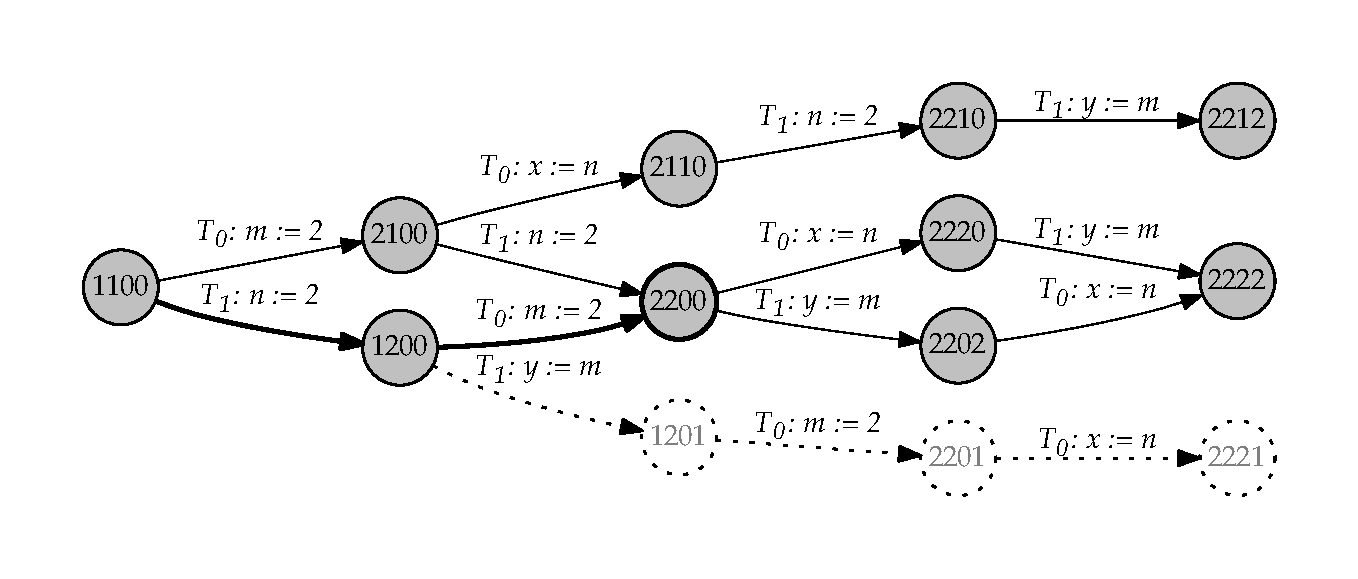
\includegraphics[width=\textwidth]{sdpor}
	\end{subfigure}
	\caption[An example illustrating the need for the
		Stateful DPOR algorithm.]
		{An example showing that na\"{\i}vely
		cutting short the DPOR algorithm is
		unsound. Each state in the diagram shows
	the values of \textit{mnxy}.}
	\label{fig:sdpor-motivation}
\end{figure}

\subsubsection{Stateful Dynamic Partial-Order Reduction}
The most obvious solution to this problem is to simply
add all possible backtracking points whenever we cut
short a search. Although this does guarantee that all
necessary backtracking points are added (and therefore
that the algorithm is sound), in practice, the cost
of exploring \emph{all} possible previous backtracking points
dominates the benefit of cutting short searches when we
encounter an already-visited state. To make use of this
technique, we need a method of conservatively deciding which
backtracking points must be added for soundness, but not
so conservatively that all practical benefits are lost.

One such method is to use a \emph{visible operation dependency
graph}, and its use was proposed by \textbf{names} in an
algorithm which is known as Stateful Dynamic Partial-
Order Reduction (SDPOR). The idea is that, when we first explore
a section of the state space,
we make a note of the visible operations
that may be executed, so that if we encounter that section again,
we can cut short the search, and use our knowledge of the
visible operations that may have been
executed if the search was continued
to add backtracking points as necessary.

In particular, a \emph{visible operation dependency
graph} is a graph $G = \langle V, E \rangle$ whose
nodes represent visible operations, and whose edges
represent the ordering of those transitions; whenever
a transition sequence of the form
$\sigma_1 \xrightarrow{t} \sigma_2 \xrightarrow{t'}
 \sigma_3$
is encountered in a search of the state space, the
edge $(t, t')$ is added to the visible operation
dependency graph $G$. Then, when a state $\sigma$ is
encountered which has already been explored on the
search, sufficient backtracking points for soundness
can be added by calling the
\textsc{UpdateBacktrackSets} procedure
on each transition in the set
$\mathcal{U} = \{u \mid \exists t \in \textit{enabled}(\sigma).\;
   u \text{ is reachable from node } t \text{ in graph } G\}$.
The assumption that Stateful DPOR algorithm 
relies on fir its efficiency is that
although state spaces are generally very large,
the sets $\mathcal{U}$ of reachable transitions
are generally small.

The pseudocode for the SDPOR algorithm is shown
in figure~\ref{fig:sdpor-code}. The lines that
differ from the plain DPOR algorithm are lines
6--10 and line 19.
To implement the visible operation dependency graph
$G$, I chose to use another hash table,
mapping from transitions to lists of transitions.
Calling \textsc{UpdateBacktrackSets} on
each reachable node in $G$ is implemented using
a simple depth-first search.

\begin{figure}
	\begin{algorithmic}[1]
		\Let{$H$}{an empty hash table of states}
		\Let{$G$}{an empty graph on transitions}
		\State
		\Procedure{Explore}{$\pi$}
		\Let{$\sigma$}{$\textit{last}(\pi)$}
		\If{$\sigma \in H$}
			\Let{$\mathcal{U}$}
			{$\{u \mid \exists t \in \textit{enabled}(\sigma).\;
				u \text{ is reachable from node }
				t \text{ in } G\}$}
			\ForAll{$t \in \mathcal{U}$}
			\Call{UpdateBacktrackSets}
				{$\pi,\, t$}
			\EndFor
		\Else{
		\State add $\sigma$ into $H$;
		\ForAll{$p \in \mathcal{P}$}
		\Call{UpdateBacktrackSets}
		{$\pi,\, \textit{next}(\sigma, p)$};
		\EndFor
		\If{$\textit{enabled}(\sigma) \neq \emptyset$}
		\Let{$t$}{any $t \in \textit{enabled}(\sigma)$}
		\Let{$\textit{backtrack}(\sigma)$}{$\{t\}$}
		\Let{$\textit{done}(\sigma)$}{$\emptyset$}
		\While{$\textit{done}(\sigma)
			\neq \textit{backtrack}(\sigma)$}
		\Let{$t$}{any $t \in (\textit{backtrack}(\sigma)
			\setminus \textit{done}(\sigma))$}
		\State add $t$ to $\textit{done}(\sigma)$;
		\If{$|\pi| > 0$}
			add edge $(\pi_{|\pi|-1}, t)$ to $G$;
		\EndIf
		\State \Call{Explore}{$\pi.t$}
		\EndWhile
		\EndIf
		}\EndIf
		\EndProcedure
		\State
		\Procedure{UpdateBacktrackSets}{$\pi,\, t_{p,s}$}
		\Let{$D$}{$\{i \in \textit{dom}(\pi) \mid
			\pi_i \text{ is dependent with } t_{p,s}
			\text{ and } (i, p)\!\not \hookrightarrow_\pi \}$}
		\If{$D \neq \emptyset$}
		\Let{$\sigma_d$}
		{$\textit{pre}(\pi,\text{max}(D))$}
		\If{$\textit{next}(\sigma_d, p)
			\in \textit{enabled}(\sigma_d)$}
		add $\textit{next}(\sigma_d, p)$
		to $\textit{backtrack}(\sigma_d)$
		\Else {
			add all of $\textit{enabled}(\sigma_d)$
			to $\textit{backtrack}(\sigma_d)$
		} \EndIf
		\EndIf
		\EndProcedure
		\State
		\State Initially: \Call{Explore}{$\emptyset$}
	\end{algorithmic}
	\caption{The Stateful DPOR algorithm.}
	\label{fig:sdpor-code}
\end{figure}

\section{Static Partial-Order Reduction}
After reading this section, you should
understand the static partial-order
reduction algorithm that I implemented,
and also why I did not implement a
published static partial-order reduction
algorithm.

In order to evaluate the improvement in performance
allowed by building persistent sets dynamically
instead of statically, I decided to research and
implement a static partial-order reduction
algorithm. However, I struggled to find one
in the literature that was straightforward enough
to understand and implement in the short amount
of time I had. I therefore designed my own
rudimentary static partial-order reduction algorithm,
which I will refer to at the Static POR (SPOR,
not to be confused with SDPOR) algorithm.
While it is simple to understand and implement,
the trade-off is that it returns large persistent sets.

The algorithm explores the state space using a
depth-first search, but exploring only those
transitions in a persistent set from each
state, as mentioned in section \ref{sec:persistent}.
Before the algorithm begins its search, it compiles a table
listing all the shared objects that each process may
access, then, during the search, persistent sets $T$ are built
using a fixed-point computation such that
every process whose next transition is
not in $T$ never accesses any
object that any process whose next
transition is in $T$ accesses.
The algorithm constructing a persistent set in a given state
is shown in figure~\ref{fig:spor-code}.

\begin{figure}
	\begin{algorithmic}[1]
		\Procedure{PersistentSet}{$\sigma$}
		\Let{$E$}{$\{p\}$,
			for any $p$ such that
			$\exists t_{p,s} \in \textit{enabled}(\sigma)$}
		\Let{$O$}{$\{o \mid \textit{accesses}(p, o)\}$}
		\While{$E$ changes}
			\ForAll{$q \in (\mathcal{P} \setminus E)$}
				\If{$\exists o \in O.\;
					\textit{accesses}(q,o)$}
				\State $E := E \cup \{p\}$;
				\State $O := O \cup \{o \mid
					\textit{accesses}(q, o)\}$
				\EndIf
			\EndFor
		\EndWhile
		\Let{$T$}{$\{t \mid \exists p \in E.\;
					t = \textit{next}(\sigma,p)\}$}
		\If{$(T \setminus \textit{enabled}(\sigma))
				\neq \emptyset$}
			\Return $\textit{enabled}(\sigma)$
		\Else \ \Return $T$
		\EndIf
		\EndProcedure
	\end{algorithmic}
	\caption{An algorithm for statically constructing
		persistent sets.}
	\label{fig:spor-code}
\end{figure}

\section{Sleep Sets}
After reading this section, you
should understand how I implemented
the sleep sets technique for both the
simple model checking algorithm and
the dynamic partial-order reduction
algorithm.

\begin{figure}
	\begin{algorithmic}[1]
		\Let{$H$}{an empty hash table mapping
			states to sets of transitions}
		\State
		\Procedure{Check}{$\sigma,\, \textit{Sleep}$}
			\If{$\sigma \not \in H$}
				\State add $(\sigma, \textit{Sleep})$ to $H$
				\State$T := \textit{enabled}(\sigma)
					\setminus \textit{Sleep}$
			\Else
				\State$T := H(\sigma) \setminus
					\textit{Sleep}$
				\State $\textit{Sleep} := \textit{Sleep}
					\cap H(\sigma)$
				\State $H(\sigma) := \textit{Sleep}$
			\EndIf
			\ForAll{$t \in T$}
				\Let{$\sigma'$}{$\sigma'$ such that
					$\sigma \xrightarrow{t} \sigma'$}
				\Let{$\textit{Sleep}'$}{$\{t' \in \textit{Sleep}
					\mid t' \text{ is independent with } t\}$}
				\State\Call{Check}{$\sigma',\, \textit{Sleep}'$}
			\EndFor
		\EndProcedure
		\State
		\State Initially: \Call{Check}{$\sigma_0,\, \emptyset$}
	\end{algorithmic}
	\caption{Simple model checker with sleep sets}
	\label{fig:sleep-code}
\end{figure}

\section{Counter-Example Traces} \label{sec:traces}
After reading this section, you should understand
how I implemented a feature which produces a
visual counter-example trace.

One of the advantages of model checking
is that, in the case that
an error is found, it is trivial to give
an example of an execution of the given
program which leads to an error state---in
our case, this is just the sequence of
transitions executed at the point when
an error state it found.
To give more insight into the reason for the
error state being entered, it would be preferable
to instead present the user with a
\emph{partial order} of the transitions which,
whenever linearised in an execution,
results in the error/deadlock state.
Given a sequence of transitions which lead to
some state of interest, the problem is
then to give the most general partial order
which, however linearised, results a sequence
of transitions that leads to the same error
state.

This partial order is simply the happens-before
relation, as described in
section~\ref{sec:happens-before}). As
two transitions are dependent if and only
if they belong to the same thread or if
they access the same shared object, my
algorithm simply executes the given transition
sequence, using a function from processes
to sequence indices to keep track
of the last transition to access each
process, and a function from shared
objects to sequence indices to keep
track of the last transition to
access each shared object. For each
transition executed, two edges are added
to the graph representing the partial
order: one from the last transition
belonging to the same process, and one
from the last transition accessing the
same shared object.

I thought that the most helpful way to
present the resulting partial-order
graph would be in the form of an
image, so I wrote a function which
automatically output the graph as
a GraphViz graph, with the nodes
labelled with the thread and the
shared object accessed of each transition.
GraphViz is an open-source program which
draws graphs.
Figure~\ref{fig:trace-example} gives a program
and shows an example of such an
automatically-generated GraphViz graph.

\begin{figure}
	\centering
	\begin{subfigure}{0.5\textwidth}
		\centering
		\begin{tabular}{l}
			Shared variables: \\
			\qquad \texttt{n}, \texttt{w},
			\texttt{x} and \texttt{y},
			initially \texttt{0} \\
			\qquad \texttt{t} and \texttt{z},
			initially \texttt{false} \\
			\\
			Thread 0: \\
			\qquad \texttt{t := z;} \\
			\qquad \texttt{if t then x := y} \\
			\\
			Thread 1: \\
			\qquad \texttt{n := 1;} \\
			\qquad \texttt{z := true} \\
			\\
			Thread 2: \\
			\qquad \texttt{y := 2;} \\
			\qquad \texttt{if w = 1 \& x = 2 then \textbf{error}} \\
			\\
			Thread 3: \\
			\qquad \texttt{w := n} \\
			\\
			Thread 4: \\
			\qquad \texttt{t := false} \\
		\end{tabular}
	\end{subfigure}%
	\begin{subfigure}{0.5\textwidth}
		\centering
		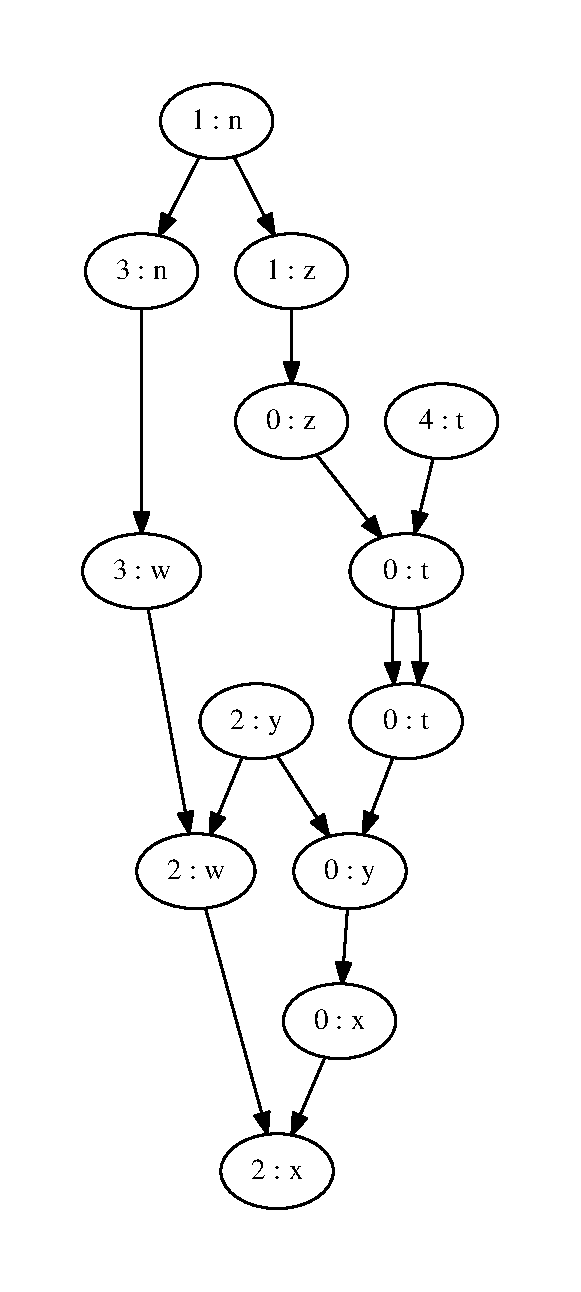
\includegraphics[height=15cm]{error_trace}
	\end{subfigure}
	\caption[An example partial-order
		error trace.]{An example partial-order
			error trace. The two nodes marked
			``0 : t'' have two edges between them
			as their happens-before relationship
			is due to both possible reasons:
			belonging to the
			same process and accessing the same
			shared object. The assignments in
			the program are implemented in PL
			using compare-and-swap operations.}
	\label{fig:trace-example}
\end{figure}

\section{Summary}
Having read this chapter,
you should now understand:
\begin{understandinglist}
	\item that I used OCaml modules to
	structure my project, making
	particular use of functors to generate
	code that implements different model-checking
	algorithms on a given language implementation;
	\item that I used an iterative development
	process to first implement the project
	language (PL), then to implement the simple
	model-checking algorithm, then
	the DPOR algorithm, and then extend the project
	with extra algorithms and features; and
	\item the details of my
	implementations of PL and the
	model-checking algorithms.
	\end{understandinglist}

\chapter{Evaluation}
\label{cha:evaluation}

After reading this chapter,
you should understand:
\begin{understandinglist}
	\item the extent to which I believe
	the project is correct, and the evidence
	motivating that belief;
	\item that being certain of the
	correctness of a model checking
	system is not essential for it
	to be of practical use;
	\item how my implementations
	of the model-checking algorithms
	perform, in terms of their
	execution times;
	\item how the model-checking
	algorithms themselves perform
	in comparison to one another,
	in terms of the reduction in the
	size of the explored state space; and
	\item the relationship between the
	inherent complexity of the
	algorithms and the performance of
	my implementations of them.
\end{understandinglist}

\section{Soundness}

\begin{center}
	\textit{But who will guard the guards themselves?} \\
	\qquad\qquad\qquad --- Juvenal, \textit{Satire VI}
\end{center}

Even though the algorithms
used in this project have all been proven sound,
there is no guarantee that my project correctly
implements the algorithms, and hence no
guarantee of soundness. Using another
system to verify
my model-checking implementations would not
solve this problem, because then that system
would have to be verified, and so on.
After reading this section, you should
therefore understand the extent to which I believe
my project consists of sound implementations
of the model-checking algorithms, the
evidence leading to this belief, and why
model checking systems are useful in
practice without being known to be
sound.

\subsection{Evidence for Soundness}
While any program of a reasonable size
is extremely likely to contain bugs
\textbf{[citation]}, I believe that
on the balance of probabilities,
all remaining bugs in my project will
probably relate
to functionality not necessary for
soundness. For instance, I would
not be surprised to learn that there
is a bug in the \texttt{next\_transition}
function for PL, whereas I would be
surprised if such a bug existed in
my implementation of the DPOR
algorithm. There are two main reasons
for this belief: my testing process,
and my understanding of the
algorithms involved.

\subsubsection{Examination of Source Code}
OCaml is a very high-level language, so
its use allowed me to keep the source code
relatively simple. As a result,
the correspondence between
the published pseudocode for an algorithm
and my source code implementing it was
as clear as possible, meaning that it
is possible to convince yourself that
the implementation is correct by simply
comparing the two. In the development
process, I spent a lot of time trying
to find ways in which my programs did
not match the pseudocode; at the end
of the development process, I can be
reasonably confident that any differences
in semantics
(apart from perhaps very subtle ones)
have been found. This is especially
true for the simple model checker,
due to its simplicity.

\subsubsection{Tests}
\label{sec:pl-checker-tests}
As part of the development process,
I wrote over forty test cases, each
consisting of a transition system
implemented as a PL program, and
the expected
$(\textit{error-free},\, \textit{deadlock-free})$
result of model checking that program.
Running an implementation of a
model-checking algorithm on the
program should give the expected
result: if not, then either
the result I expected was wrong
(usually due to an incorrect encoding
of the transition system in PL),
or the implementation was incorrect.
To ensure the former was not a possibility,
I used the simple model checker---whose
correctness I have a lot of confidence in due
to its simplicity---to check that my
expectations of the results were correct.

The primary use of these tests was to
reveal the presence of bugs in my
project during its development, so
that I could track them down and
remove them. However, they have the
secondary benefit of providing
evidence that my implementations are
correct: if a bug is not applicable
in any of the test cases, then,
assuming that these test cases cover a
varied and representative selection
of systems to be verified,
the bug must be very obscure.

\subsection{Model Checking In Practice}
Even if I think it is unlikely, it is
certainly possible that there is a subtle
bug in my project which results in its
unsoundness; it may report a transition system
to be error- and deadlock-free when it
is not. In fact, since any verification
system can only be verified (with considerable
effort) with another
automated verification system, it is
more or less impossible to be \emph{certain}
of the correctness of any model checker.
Although it may initially seem
that such a model checking system without
rigorous, unshakeable proof of its
soundness is useless, this
is not at all the case.

\subsubsection{Proofs of Soundness are Unnecessary}

What is a proof of soundness, anyway?
A distinction can be made between two
main notions of proof \cite[p.~2]{buss98}:
\begin{enumerate}
	\item a (social) proof is an argument
	designed to convince human readers that some
	result is true and ideally create a consensus
	in the relevant community, and
	\item a (formal) proof is a sequence of
	symbols, which, according to a particular
	set of formal rules, lead to some
	theorem, another sequence of symbols.
\end{enumerate}
I would argue that the former is the far more
relevant notion when considering the
correctness of a model-checking implementation,
since the end goal is a consensus that the
system is correct.
There are several reasons that obtaining a formal
proof of the correctness of my project,
produced by some other verification system,
would not be as useful as you might think:
\begin{itemize}
	\item the proof would be impractically
	long to read and verify by hand, and so
	would do little to convince a human reader
	of the project's soundness, which is the real
	goal;
	\item there are easier ways of increasing
	confidence in the correctness of the system,
	such as running tests, gaining 
	experience from long-term use, and
	especially performing cross-checking
	with other,
	independently developed
	model-checking implementations \cite{tau02};
	\item a verified project may still be
	unsound in practice, due a bug
	in the compiler, operating system or
	hardware; and
	\item other aspects of the project,
	such as efficiency and usability, are
	more important than soundness, since
	a partially-correct system can still
	be used to find bugs, whereas an
	unusable system or a system that
	cannot tackle realistic problems
	cannot.
\end{itemize}

The lack of need for formal verification of
verification systems is evident in
practice---Isabelle, for instance, is widely
believed to be correct even thought its
implementation is not verified, and
as of 2006, there were only
two verified model checking
systems, neither of which was widely
used \cite{beck06} (despite model
checking having been around for
over two decades). 

\subsubsection{Model Checking as Rigorous Testing}
The value in an unverified model-checking system
is clear when thought about in relation to testing.
Model checking provides full coverage of the code,
covering every possible behaviour case; in particular,
bugs due to race conditions in concurrent software
are notoriously difficult to expose using normal
testing, but model checking is designed with such
bugs in mind. Furthermore,
it is fully automatic, whereas writing \textit{ad hoc}
tests by hand, especially if aiming
for full code coverage or trying to discover
concurrency bugs, takes time.
When a bug \emph{is} found, model checking
provides information that is likely to lead the
developer to immediately identify its cause.
here have been many examples of serious bugs
which have been found using model checking
which would not have been found until much
later otherwise.

Perhaps the best argument for the practical
benefits of model checking, (without the
model checker being verified)
is the many cases where the technique has
discovered bugs in real applications which
had been missed by the normal testing
process. \textbf{Give references)}

\section{Performance}
\textbf{This section compares the
	performance of the various algorithms
	in the project. This is achieved by
	looking at execution times, transitions
	explored, and numbers of states explored
	while model checking various example
	programs. Comparison can be made with
	published figures.}

\begin{itemize}
	\item The performance depends strongly
	on the program being checked, so that
	analysing is difficult: there is no
	obvious ``average case"
	\item We will instead use several
	benchmarks published in the literature
	for analysis of model checking performance
	\item As well as comparing the various
	algorithms to each other, I will also
	compare with published results
	\item Transitions are one measure of
	performance: the reduction in the size
	of the state space is a property of the
	algorithm, not the implementation, 
	assuming the implementation is correct
	\item (In fact transitions can therefore
	be used as evidence for correctness)
	\item Execution time is another measure
	of performance: the relationship between
	execution time and transitions explored
	gives information about both the
	intrinsic complexity of the algorithm
	and specifically the efficiency of my
	implementation. Separating these two
	aspects will be done below.
	\item Analysis will be done of the above
	things as a function of number of threads,
	and amount of computation in each thread.
\end{itemize}

\subsection{Performance of Algorithms}

\begin{figure}
	\newenvironment{figtile}
		{\begin{subfigure}{0.48\textwidth}
			\def\svgwidth{\textwidth}
			\captionsetup{font=footnotesize}
		}
		{\end{subfigure}}
	\centering
	\footnotesize
	\begin{figtile}
		\input{figs/t43_tpl1_ops1.pdf_tex}
		\caption{1 thread per location,
			each of 1 operation.}
	\end{figtile}%
	\quad
	\begin{figtile}
		\input{figs/t43_tpl1_ops3.pdf_tex}
		\caption{1 thread per location,
			each of 3 operations.}
	\end{figtile}
	\begin{figtile}
		\input{figs/t43_tpl2_ops1.pdf_tex}
		\caption{2 threads per location,
			each of 1 operation.}
	\end{figtile}%
	\quad
	\begin{figtile}
		\input{figs/t43_tpl2_ops3.pdf_tex}
		\caption{2 threads per location,
			each of 3 operations.}
	\end{figtile}
	\begin{figtile}
		\input{figs/t43_tpl3_ops1.pdf_tex}
		\caption{3 threads per location,
			each of 1 operation.}
	\end{figtile}%
	\quad
	\begin{figtile}
		\input{figs/t43_tpl3_ops3.pdf_tex}
		\caption{3 threads per location,
			each of 3 operations.}
	\end{figtile}
	\begin{figtile}
		\input{figs/t43_tpl4_ops1.pdf_tex}
		\caption{4 threads per location,
			each of 1 operation.}
	\end{figtile}%
	\quad
	\begin{figtile}
		\input{figs/t43_tpl4_ops3.pdf_tex}
		\caption{4 threads per location,
			each of 3 operations.}
	\end{figtile}
	\caption{Graphs showing test 43 transitions explored.}
\end{figure}

\begin{figure}
	\newenvironment{figtile}
	{\begin{subfigure}{0.48\textwidth}
			\def\svgwidth{\textwidth}
			\captionsetup{font=footnotesize}
		}
		{\end{subfigure}}
	\centering
	\footnotesize
	\begin{figtile}
		\input{figs/t43_time_tpl1_ops1.pdf_tex}
		\caption{1 thread per location,
			each of 1 operation.}
	\end{figtile}%
	\quad
	\begin{figtile}
		\input{figs/t43_time_tpl1_ops3.pdf_tex}
		\caption{1 thread per location,
			each of 3 operations.}
	\end{figtile}
	\begin{figtile}
		\input{figs/t43_time_tpl2_ops1.pdf_tex}
		\caption{2 threads per location,
			each of 1 operation.}
	\end{figtile}%
	\quad
	\begin{figtile}
		\input{figs/t43_time_tpl2_ops3.pdf_tex}
		\caption{2 threads per location,
			each of 3 operations.}
	\end{figtile}
	\begin{figtile}
		\input{figs/t43_time_tpl3_ops1.pdf_tex}
		\caption{3 threads per location,
			each of 1 operation.}
	\end{figtile}%
	\quad
	\begin{figtile}
		\input{figs/t43_time_tpl3_ops3.pdf_tex}
		\caption{3 threads per location,
			each of 3 operations.}
	\end{figtile}
	\begin{figtile}
		\input{figs/t43_time_tpl4_ops1.pdf_tex}
		\caption{4 threads per location,
			each of 1 operation.}
	\end{figtile}%
	\quad
	\begin{figtile}
		\input{figs/t43_time_tpl4_ops3.pdf_tex}
		\caption{4 threads per location,
			each of 3 operations.}
	\end{figtile}
	\caption{Graphs showing test 43 execution times.}
\end{figure}

\begin{figure}
	\centering

	\def\svgwidth{15cm}
	\input{figs/prod_cons_trans_fig.pdf_tex}
	\caption{Producer-Consumer transition graph.}

	\def\svgwidth{15cm}
	\input{figs/prod_cons_time_fig.pdf_tex}
	\caption{Producer-Consumer time graph.}
\end{figure}
\begin{figure}
	\def\svgwidth{15cm}
	\input{figs/fs_trans_fig.pdf_tex}
	\caption{File system transition graph.}

	\def\svgwidth{15cm}
	\input{figs/fs_time_fig.pdf_tex}
	\caption{File system time graph. See above for key.}
\end{figure}
\begin{figure}
	\centering

	\def\svgwidth{15cm}
	\input{figs/indexer_trans_fig.pdf_tex}
	\caption{Indexer transition graph. See above for key.}

	\def\svgwidth{15cm}
	\input{figs/indexer_time_fig.pdf_tex}
	\caption{Indexer time graph. See above for key.}
\end{figure}
\subsubsection{Comparison with Each Other}
Here, we will analyse the reduction in the size of the
state space that each model checking algorithm
offers in comparison to the simple model checker.
\subsubsection{Comparison with Published Results}

\subsection{Execution Times of Model Checking}
\subsubsection{Comparison with Each Other}
\subsubsection{Comparison with Published Results}

\section{Summary}
Having read this chapter,
you should now understand:
\begin{understandinglist}
	\item the extent to which I believe
	the project is correct, and the evidence
	motivating that belief;
	\item that correctness is not
	essential for a model-checking
	system to be of practical use;
	\item how my implementations
	of the model-checking algorithms
	perform, in terms of their
	execution times;
	\item how the model-checking
	algorithms themselves perform
	in comparison to one another,
	in terms of the reduction in the
	size of the explored state space; and
	\item the relationship between the
	inherent complexity of the
	algorithms and the performance of
	my implementations of them.
	\end{understandinglist}
\textbf{TO DO: update these with summaries.}

\chapter{Conclusions}

\textbf{This chapter makes some
	interesting conclusions, which I
	haven't thought of yet.}


%%%%%%%%%%%%%%%%%%%%%%%%%%%%%%%%%%%%%%%%%%%%%%%%%%%%%%%%%%%%%%%%%%%%%
% the bibliography
\addcontentsline{toc}{chapter}{Bibliography}
\bibliography{refs}

%%%%%%%%%%%%%%%%%%%%%%%%%%%%%%%%%%%%%%%%%%%%%%%%%%%%%%%%%%%%%%%%%%%%%
% the appendices
\appendix

\chapter{PL Definition}
 
\textbf{This will be the definition
	of PL.}
 
\chapter{Example PL Programs}

\textbf{This will contain various
	example programs, in particular
	those used for performance evaluation.}

\chapter{Project Proposal}

Project proposal here
% \input{proposal_without_title}

\end{document}
